\chapter{Monotonicity preserving methods for continuous Galerkin method}
\label{chap-paper1}
\section{Introduction}\label{s-intro}
%
%In this work, we design stabilized finite element (FE) approximations of hyperbolic problems
%with monotonicity properties, which also serve to solve singular limits of 
%convection-diffusion-reaction problems. We focus on the linear tranport equation
%and the nonlinear Burgers equation.

The finite element (FE) Galerkin approximation of convection-dominated and transport problems
with non-smooth data produces highly oscillatory results, and additional numerical stabilization must be
introduced. The most rudimentary stabilization methods add non-consistent terms, e.g., homogeneous artificial diffusion and upwinding techniques \cite{von_neumann_method_1950}. 
The SUPG method originally proposed in \cite{brooks_streamline_1982} was the first consistent stabilization technique, 
allowing for higher order approximations. Since this groundbreaking
work, the amount of research produced on linear stabilization has been impressive, leading to a wide 
variety of formulations (see, e.g., \cite{hughes_variational_1998,codina_finite_1997,becker_finite_2001,guermond_stabilization_1999}). 
%Remarkable works are the concept of subgrid stabilization in \cite{}, the variational
%multiscale paradigm in \cite{hughes_variational_1998} or the symmetric projection stabilization techniques in \cite{codina_finite_1997,becker_finite_2001}.

We can roughly distinguish between linear stabilization methods based on FE residuals 
and methods based on projections. Residual-based methods include the
SUPG, GLS, and VMS formulations \cite{hughes_multiscale_1995,hughes_variational_1998} proposed by Hughes and co-workers. These
methods are consistent by definition and exhibit optimal convergence and stability properties.
However, these methods can be cumbersome for complex systems of equations, specially
in multiphysics \cite{planas_approximation_2011,badia_unconditionally_2013}, where the number of stabilization terms to be integrated 
notably increases; only some terms do introduce stability whereas the rest are only required
to keep consistency. These additional terms can couple unknowns that are uncoupled
at the con\-ti\-nuous level, destroy symmetric properties and  make unstable segregated
algorithms \cite{badia_unconditionally_2013}. Furthermore, the extension of these methods to transient problems is
involved unless space-time discretizations are considered \cite{codina_time_2007,burman_consistent_2010}. 


% Modify the sentece since the introduction
% In fact, for the sake of convergenge, only the projection orthogonal to the FE space is used.
In order to solve all these problems, symmetric projection stabilization only introduces the terms that are required for stability purposes. More specifically, it only provides stability of the projection orthogonal to the FE space, so that the stabilization terms do not spoil the convergence of the method. %Since the introduction of the whole quantities to be stabilized, e.g. the convective term, would spoil convergence, the projection of these quantities onto the corresponding FE space is subtracted.  
This way, we keep convergence and attain the desired stability, e.g., relying on continuous inf-sup conditions. The key aspect of these methods is the choice of the projector. One example  is the orthogonal subscales method in \cite{codina_stabilization_2000}, which uses a (global) $L^2$ projection. In order to avoid the need of a global projection, local projection stabilization techniques have been proposed, e.g., in \cite{braack_local_2006,matthies_unified_2007}. The resulting methods only involve local projections but are restricted to particular mesh topologies or require enriched FE spaces. A recent improvement of these formulations has been recently proposed in \cite{badia_stabilized_2012} for pressure stability of the Stokes problem, which makes use of  a particular Scott-Zhang projector which is local and does not require any particular type of mesh or FE space enrichment; this method has been named \emph{nodal projection stabilization} (NPS), due to the nodal-wise nature of the projection. A closely related term-by-term pressure/convection stabilization has been presented in \cite{rebollo_high_2013}. The main difference between the stabilization mechanism in \cite{badia_stabilized_2012} and  \cite{rebollo_high_2013} is the \emph{buffer} FE space in which the projections are performed. The buffer space in \cite{badia_stabilized_2012} is the same velocity FE space, whereas  it has one order less than the velocity space (assumed to be at least quadratic) in \cite{rebollo_high_2013}.

 %This method coincides with the nodal interpolation proposed by Chac\'on \textit{et al.} in \cite{rebollo_high_2013}.


Linear stabilization certainly reduces oscillations but still exhibits overshoots and undershoots around discontinuities or shocks. As a result, nonlinear stabilization techniques (traditionally called shock-capturing) have been designed, usually in the form of an artificial viscosity that depends on the solution (see, e.g., \cite{johnson_convergence_1987,johnson_convergence_1990,szepessy_convergence_1989}). This nonlinear viscosity must be active around shocks, where it sacrifices the order of accuracy of the method but improves stability. The way this artificial viscosity is computed leads to different families of methods. Most methods are based on residual-based viscosity \cite{codina_stabilization_2000,lube_residual-based_2006,john_spurious_2007,john_spurious_2008} combined with linear stabilization. Guermond and co-workers have proposed entropy-viscosity methods, %have recently been proposed by Guermond and co-workers,
 in which the nonlinear viscosity is defined in terms of some entropy inequality \cite{guermond_entropy_2011}. %Convergence analysis and monotonic properties of EV methods are an open problem.

The aim of the nonlinear stabilization is to eliminate oscillations around shocks, which implies to satisfy a discrete maximum principle (DMP). Only a few FE methods are known to satisfy some monotonicity property (see, e.g., \cite{mizukami_petrov-galerkin_1985,burman_nonlinear_2002,burman_stabilized_2005}). It is remarkable the work by Burman and Ern in \cite{burman_nonlinear_2002}, where they state the properties to be fulfilled by a method in order to satisfy a DMP property in a useful variational setting for nonlinear problems. The methods in \cite{burman_stabilized_2005,burman_edge_2004} satisfy a DMP property for the steady-state convection-diffusion-reaction (CDR) problem but it has been observed that they are too dissipative for practical use in \cite{john_spurious_2008} and the extension to time-dependent problems is unclear. Afterwards, Burman has proposed in \cite{burman_nonlinear_2007} a method which only includes nonlinear stabilization and satisfies monotonicity properties for the (transient) Burgers' problem in one dimension. %Another approach is the ??? method  by Kuzmin, %which essentially modifies the resulting matrix in order to attain the DMP property.  
Existence and uniqueness have been proved for some residual-based shock-capturing techniques combined with local
projection stabilization via Lipschitz continuity and Brouwer's fixed point theorem in \cite{barrenechea_local_2013}.

%the resulting method satisfies a DMP but it has been observed
%to be too dissipative for practical use in \cite{}. In \cite{}, 

The combination of linear and nonlinear stabilization seems to be the winning choice, since the former is an accurate method with optimal convergence properties that is effective on smooth regions whereas the latter reduces (or eliminates) oscillations around shocks or discontinuities. In par\-ti\-cular, when using nonlinear artificial viscosity without any linear stabilization, it is common to observe the \emph{terracing effect}, which consists in ``a distortion of smooth profiles and represents an integrated, nonlinear effect of residual phase error'' \cite{kuzmin_flux-corrected_2005,oran_numerical_2005}. However, the combination of linear
and non\-li\-near stabilization must be carried out with care. A naive combination of an 
optimally convergent linear stabilization and a monotonicity-preserving nonlinear
stabilization can produce a method with none of these properties. It has recently been 
observed in \cite{ern_weighting_2012} that traditional linear stabilization terms usually harm interesting properties of the nonlinear stabilization, since they act as a hyperviscosity term. In \cite{ern_weighting_2012}, the authors propose a way to blend edge stabilization  \cite{burman_edge_2004} with entropy-viscosity and numerically observe that the resulting method converges to entropy
solutions; neither a DMP nor entropy stability is proved.

In this chapter we introdue a linear/nonlinear stabilized FE formulations to approximate hyperbolic problems (and by extension singular limits of CDR systems). The outcomes of this research are:
\begin{itemize}
\item  We extend the NPS technique proposed in \cite{badia_stabilized_2012} for pressure stabilization to convection stabilization. We carry out the stability and convergence analysis, getting full control on the convection term (times a stabilization parameter).\footnote{This is an improvement of our analysis with respect to the one in \cite{rebollo_high_2013} for a similar formulation, which only provides partial control over convection, i.e., the component orthogonal to the FE space with respect to the aforementioned projector. However, the analysis in \cite{rebollo_high_2013} is not restricted to quasi-uniform meshes.}
\item Next, we show how to weight this linear stabilization in such a way that it  does not affect the potential  monotonicity of the underlying method. The use of the Scott-Zhang projector in the NPS stabilization turns out to be essential to design a linear stabilization that allows one to preserve DMP properties. 
\item 
Then we present some nonlinear stabilization, i.e., shock-capturing, methods with some  monotonicity properties. In particular, we design a method that enjoys a DMP for time-dependent multidimensional linear transport problems. 
%\item One of those methods is defined for the 1$D$ Burgers' equation and it is proved in  \cite{burman_nonlinear_2007} that it is not only monotonic but also entropy stable; thus an alternative blending between this nonlinear stabilization and the Scott-Zhang term is proposed in order to ensure that the combination mantains entropy stability.  
\item   We present a detailed numerical experimentation, where we show the excellent performance of the proposed algorithms in terms of elimination of oscillations, compared to some up-to-date shock-capturing schemes. 
%Using numerical experimentation, we show that one of the novel shock capturing techniques proposed in this work, %which can be considered a multidimensional extension of the one in \cite{burman_nonlinear_2007}, 
%produces results superior to any of the best up-to-date schemes, since it is provably monotonic. % (see \cite{john_spurious_2007,john_spurious_2008}). 
\end{itemize}


The outline of the chapter is the following. In Section \ref{s-prel} we introduce the continuous problems and its
Galerkin discretization using FEs. Section \ref{s-fem} is devoted to the NPS formulation based on the Scott-Zhang projector and its corresponding numerical analysis. Section \ref{s-weightDMP} proposes a weighting of the previous linear stabilization in order to not affect the monotonicity of the underlying method. Novel nonlinear stabilization techniques are introduced in Section \ref{s-nonstab}. A summary of the linear/nonlinear schemes used in the numerical experimentation, including the ones introduced in this chapter, can be found in Algorithm \ref{alg-wNPS-GJV}. Numerical experiments are included in Section \ref{s-numex}. Finally, some conclusions are drawn in Section \ref{s-concl}.


\section{Preliminaries}\label{s-prel}

Let us consider an open, bounded, and Lipschitz  polyhedral domain $\Omega \subset \mathbb{R}^d$, where $d = 1,\, 2$, or $3$ is the space dimension, and a time interval $(0,T)$. The linear transport problem consists in finding a solution $u(x,t)$ for the problem
\begin{equation}\label{eq-probcont}
\partial_t u +   \nabla \cdot (\beta u) = f, \qquad \hbox{ in } \ \Omega \times (0,T),
\end{equation}
where $\beta$ is a solenoidal vector field and $f$ is the forcing term. This problem is supplemented with the boundary condition $u = 0$ on the inflow boundary $\Gamma_{\rm in} := \{ x \in \partial \Omega: \, \beta(x) \cdot n(x) < 0\}$, $n$ being the outwards normal vector, and the initial condition $u(\cdot,0) = u_0$ on $\Omega$. %We define the time-space domain $Q \equiv \Omega \times (0,T)$.

We will use standard notation for Sobolev spaces (see, e.g., \cite{brezis_functional_2010}). In particular, the $L^2(\omega)$ scalar product will be denoted by $(\cdot,\cdot)_\omega$ for some $\omega \subset \Omega$, but the domain subscript is omitted for $\omega \equiv \Omega$ (analogously for the duality pairing $\langle \cdot,\cdot \rangle$). The $L^2(\Omega)$ norm is denoted by $\|\cdot\|$. 
%Similarly, the $L^\infty(\omega)$ norm will be denoted by $\|\cdot \|_{\infty,\omega}$ for any $\omega\subset\Omega$ and $\|\cdot\|_\infty$ if $\omega = \Omega$.  
We will omit the $d$ superscript in vector-valued functional spaces. In order to state the weak form of \Eq{probcont}, we introduce the spaces $H^\beta(\Omega) := \{ u \in L^2(\Omega): \,  \nabla \cdot (\beta u) \in L^2(\Omega) \}$ and $H_0^\beta(\Omega) = \{ u \in H^\beta(\Omega):\, u = 0 \, \hbox{ on } \,\Gamma_{\rm in}\}$. 

The weak form of \Eq{probcont} reads as follows: seek $u(\cdot,t) \in H_0^\beta(\Omega)$ such that $(\partial_t u,\phi) +   (\nabla \cdot (\beta u),\phi) = (f,\phi)$ for any $\phi \in L^2(\Omega)$ and almost every $t \in (0,T)$, where  $f \in L^2(\Omega)$. The well-posedness of the continuous problem relies on the following inf-sup condition (see \cite{guermond_stabilization_1999}):
\begin{align}\label{eq-infsup}
\inf_{u \in H_0^\beta (\Omega)\setminus\{0\}} \sup_{\phi \in L^2(\Omega)} \frac{(\nabla \cdot (\beta u),\phi) }{\|u\|_{H^\beta (\Omega)} \|\phi\|_{L^2(\Omega)}} \geq c_{\gamma} > 0.
\end{align}
%where the infimum is considered excluding $u = 0$.

\section{Linear stabilization}\label{s-fem}
%
%\subsection{Galerkin discretization}
Let $\mathcal{T}_h$ be a conforming and shape-regular partition of $\bar \Omega$ into $d$-simplices, quadrilaterals ($d=2$), or hexahedra ($d=3$), where every $K \in \mathcal{T}_h$ is the image of a reference element $\widehat{K}$ through an affine mapping $F_K: \widehat K \rightarrow K$ (see \cite[Chp. 2]{ciarlet_finite_2002}). %; we can assume that every edge of $\widehat{K}$ has length one.  
$P_k(\widehat K)$ is the space of complete polynomials of degree $k$ on $\widehat K$. For $d$-simplicial FE partitions, we define the space of element-wise discontinuous functions
$$
D_{h}^k := \{ v_h: v_h|_K \circ F_K \in P_k(\widehat K), \,{K} \in \mathcal{T}_h\}, \quad \hbox{ for an integer}\, k\geq 1. 
$$
The continuous FE spaces are obtained by enforcing continuity, namely $V_h^k := D_h^k \cap C^0(\bar \Omega)$. We will also make use of the FE space  $V^k_{h,0} := V^k_h \cap H_0^\beta(\Omega)$ with null trace on the inflow. For quadrilaterals and hexahedra, the spaces are obtained by replacing $P_k(\widehat K)$ by $Q_k(\widehat K)$, the space of polynomials with maximum degree $k$ in each reference space coordinate on $\widehat K$.  

Let us introduce some basic notation. Let  $q$ and $v$  be a scalar and vectorial smooth function respectively inside every element $K \in \mathcal{T}_h$. Let $K^+_\facet$ and $K^-_\facet$ be two neighboring elements and $\facet = \partial K^+_\facet \cap \partial K^-_\facet$ the corresponding common face. We denote by $q^\pm$ (idem for $v^\pm$) the trace of $q$ on $\partial K^\pm_\facet$ taken within the interior of $K^\pm_\facet$, and $n^\pm$ the outward normal to $\partial K^\pm_\facet$. We define at $\x \in \facet$ the averages and jumps 
\begin{align*}
\mean{q} := \half(q^+ + q^-),\qquad \jump{q} &:=(q^+  n^+ + q^- n^-),\\
\mean{v} := \half(v^+ + v^-) ,\qquad \jump{v} &:= (v^+ \cdot n^+ + v^- \cdot n^-).
\end{align*}


%Further, we define $\jumpt{\v} := (\v^+ \otimes \n^+ + \v^- \otimes \n^-)$.
For the FE space $V_h^k$ we denote by $\setnodes$ the set of all interpolation nodes related to $\mathcal{T}_h$ and by $\{\varphi^i_h\}_{x_i \in \setnodes}$ the corresponding nodal basis of $V_h^k$. We also denote by $\setnodes(K)$ the set of all nodes that belong to a FE $K$. Continuous FE functions can be written as $v_h = \sum_{x_i \in \setnodes} v_h^i \varphi^i_h(\x)$, where $v_h^i$ denotes the nodal value of $v_h$ corresponding to $i$. Analogously, $\{\varphi^i_h(\x)|_K\}_{K \in \mathcal{T}_h, x_i \in \setnodes(K)}$ is the basis for $D_h$ and discontinuous FE functions  are written as $v_h = \sum_{K \in \mathcal{T}_h} \sum_{x_i \in \setnodes(K)} v_h|_K^i \varphi^i_h(\x)|_K$, where $v_h|_K^i$ is the value of $v_h$ at the node $x_i$ in element $K$.  
%Further, we define the adjacency list $\mathcal{A}_h^{\rm nd}(a)$ of a node $a \in \setnodes$ as the set of nodes $c \in \setnodes$ such that $a, c\in \setnodes(K)$ for some $K \in \mathcal{T}_h$, i.e. the set of neighbor nodes. 
On the other hand, $\Omega_i$ is the set of elements $K \in \mathcal{T}_h$ such that $x_i \in \setnodes(K)$, i.e., the set of neighbor elements. Let  $h_K$ denote the diameter of $K\in\mathcal{T}_h$ and $h := \max_{K\in\mathcal{T}_h} h_K$. 

The Galerkin FE approximation of \Eq{probcont} consists in seeking $u_h \in V^k_{h,0}$ such that
\begin{equation}\label{eq-galerkin}
(\partial_t u_h,\phi_h) +   (\nabla \cdot (\beta u_h),\phi_h) =  (f , \phi_h ) , \qquad \hbox{ for any }  \ \phi_h \in V^k_{h,0}, 
\end{equation}
for almost every $t \in (0,T)$, with the initial boundary condition $u_h(0) = \pi_h(u_0)$. In the analysis of DMP properties, we will consider a Gauss-Lobatto sub-integration, denoted by $(\cdot,\cdot)_h$, of the time-derivative term, leading to a lumped mass matrix. We define as $\|\cdot \|_h$ the norm associated to the sub-integration product. The numerical experiments in Section \ref{s-numex} are carried out with and without mass lumping. For the subsequent presentation of the formulation and numerical analysis, we assume the problem is continuous in time. In the numerical experiments, we will consider both explicit and implicit time integration schemes.

Additional stabilization terms must be introduced in order to reduce the strong oscillations of the solution in \Eq{galerkin}. The SUPG method (and identically VMS or GLS residual-based stabilized formulations) applied to \Eq{galerkin} reads as follows: seek $u_h \in V^k_h$ such that
\begin{align*}%\label{eq-supg}
(\partial_t u_h,\phi_h) +   (\nabla \cdot (\beta u_h),\phi_h) &+ \sum_{K \in \mathcal{T}_h} \int_K \delta (\partial_t u_h + \nabla \cdot (\beta u_h)) \nabla \cdot (\beta  \phi_h) {\rm d} \Omega \nonumber \\ &= (f ,  \phi_h ) + \sum_{K \in \mathcal{T}_h} \int_K \delta f \nabla \cdot (\beta \phi_h) {\rm d} \Omega, \qquad \hbox{ for any }  \ \phi_h \in V^k_h, 
\end{align*}
where $\delta$ is elementwise constant with value $\delta|_K := c_{\delta} {h_K}{\| \beta \|_{L^\infty(K)}^{-1}}$ if $\| \beta \|_{L^\infty(K)}>0$ and $\delta|_K = 0$ otherwise, $c_{\delta}$ being a positive algorithmic constant ($c_{\delta} = 0.5$ in our numerical tests). The stability of this formulation has recently been proved in \cite{burman_consistent_2010} for a time-independent $\beta$, a constant in space $\delta$, and some regularity requirements. As one can observe in \cite{burman_consistent_2010}, the time derivative in the stabilization term certainly complicates the numerical analysis. An alternative to SUPG-type formulations is to use symmetric projection stabilization. 
This type of stabilization applied to problem \Eq{galerkin} admits different versions of the stabilization term, depending on the quantity that is being projected. The first version, which includes the projection of the unknown gradient/shape function, reads as:
\begin{equation}\label{eq-stproj1}
s_h(u_h,\phi_h) = ( \delta \beta \cdot \kappa_h^{\perp}(\nabla u_h), \beta \cdot \kappa_h^{\perp}(\nabla \phi_h)), 
\end{equation}
where $\kappa_h^\perp(v) = v - \kappa_h(v)$, $\kappa_h(\cdot): L^2(\Omega) \longrightarrow V^k_h$ being a projector with optimal interpolation properties. Alternatively, we can consider the projection of the whole convective term, i.e.,
\begin{equation}\label{eq-stproj2}
s_h(u_h,\phi_h) = ( \delta \kappa_h^{\perp}(\nabla\cdot (\beta u_h)),  \kappa_h^{\perp}(\nabla\cdot (\beta \phi_h)). 
\end{equation}
Both versions have a very similar numerical behaviour. In fact, they are equivalent in the case $\beta  \in V_h^1$ (linear FE space); this fact is a direct consequence of Lemma \ref{lem-kappastab}. Convergence estimates for these two versions are slightly different (see Theorems \ref{th:conv}-\ref{th:conv2}).
%From a theoretical point of view, \Eq{stproj2} provides better long-term estimates (without  

%It will be shown that the formulation \Eq{stproj1} allows one to preserve a DMP property (see Section \ref{s-weightDMP}) while \Eq{stproj2} is better to  prove long term error estimates. 
%Both formulations are equivalent in the case $\beta  \in V_h^1$ (linear FE space). If $\beta \notin V_h^1$, it will be shown that, under proper regularity conditions for $\beta$, the long term error estimates are better for the formulation \Eq{stproj2}.

Different choices of $\kappa_h$ have been proposed so far. A natural option is to consider the $L^2$ projector $\pi_h$, i.e., given $v \in L^1(\Omega)$ we compute $\pi_h(v)$ as the solution of $(\pi_h(v),\phi_h) = \langle v, \phi_h\rangle$ for any $\phi_h \in V^k_h$. However, this projector is global and cannot be straightforwardly used. Assuming $\delta$ to be constant (which is not in practical computations) the element contributions in \Eq{stproj2} are replaced by $ (\delta \pi_h^{\perp}( \beta \cdot \nabla u_h),  \beta \cdot \nabla \phi_h)$, dealing to the orthogonal subscales formulation in \cite{codina_stabilization_2000}. Still, the global projector requires the explicit computation of the inverse of a mass matrix and produces a much denser system matrix. %In order to avoid it, the projection is sent to the right-hand side via a fixed point algorithm. This approach requires an additional iterative loop to compute the orthogonal projection and is only appropriate for transient problems, when the projection is treated explicitly. %; the explicit treatment of the projection does not harm stability but couples space and time accuracy. 
Further, symmetry is lost, since $\delta$ is not constant in practice.

The local projection stabilization (LPS) in \cite{braack_local_2006} solves the aforementioned problems since this method involves a local projector; $\kappa_h$ does not project onto $V^k_h$ but a space of discontinuous functions. The original LPS method, lately called two-level LPS, requires a particular hierarchical topology of the mesh that restricts the applicability of the method. Alternative formulations have been proposed in \cite{matthies_unified_2007}, in which a fine space is obtained by including additional functions to the FE space. The resulting method, called one-level LPS, does not involve mesh restrictions but particular enriched FE spaces must be used.

We will extend the NPS method (recently proposed in \cite{badia_stabilized_2012} to attain pressure stability for the Stokes problem) to convection stabilization. We consider $\kappa_h$ to be a particular $L^1(\Omega)$ Scott-Zhang projector, which is favoured with respect to the previous symmetric stabilization techniques since \emph{only local projections} are required and neither \emph{assumptions over the mesh partition} nor \emph{enriched FE spaces} are needed. We note that the projector is locally defined at the node level, which has motivated the name of the method.


\subsection{Nodal projection stabilization}

At this point, let us introduce a variant of the Scott-Zhang projector \cite{scott_finite_1990} which is well-defined for $L^1(\Omega)$ functions. The analysis in \cite{scott_finite_1990} does apply for this projector even though it is not the standard version, because it does not keep homogeneous boundary conditions. We can build a node-to-element map $\varsigma: \setnodes \rightarrow  \mathcal{T}_h$ such that given a node $x_i$ it provides an element $K \in \Omega_i$; for interior nodes there is only one choice, two choices for nodes on faces and possibly more for nodes on edges or vertices. Following \cite{scott_finite_1990}, for any $x_i \in \setnodes$ there is only one dual function $\psi^i_h \in P_r(K)$ (analogously for $Q_r(K)$) such that
\begin{align}\label{eq-dualfunct}
\int_{\varsigma(x_i)} \psi_h^i(\x)\varphi_h^j(\x) {\rm d}\x = \delta_{ij}, \qquad \hbox{for any}\ j\in\setnodes(\varsigma(x_i)).
\end{align}
Now, we construct the projector $\kappa_h: L^1(\Omega) \rightarrow V^k_h$ as follows:
\begin{align}\label{eq-projSZ}
\kappa_h(v) := \sum_{x_i \in \setnodes}  \varphi^i_h(\x) \int_{\varsigma(x_i)} \psi_h^i(\x) v(\x) \rm{d} \x.\end{align} 
However, we can consider the following simplifications:
\begin{enumerate}
\item Since $\nabla \varphi^i_h|_K \in P_{r-1}(K) \subset P_r(K)$ for any $x_i \in \setnodes$, we can easily check that $\kappa_h(\nabla \varphi^i_h)(x_k) =  \nabla \varphi^i_h|^k_ {\varsigma(x_k)}$ and thus, to compute the stabilization term \Eq{stproj1} one \emph{does not require any integration or the explicit computation of dual functions.} 
\item We note that this trick is not possible for \Eq{stproj2} since $\beta \cdot \nabla \varphi^i_h|_K \not\in P_{r}(K)$ in general. However, we can still use the nodal projection, i.e., $\kappa_h(\beta \cdot \nabla \varphi^i_h)(x_k) =  \beta \cdot \nabla \varphi^i_h|^k_ {\varsigma(x_k)}$, keeping the required stability and approximability properties (see \cite{rebollo_high_2013}).
\end{enumerate}
We refer to \cite{badia_stabilized_2012} for a detailed discussion about implementation aspects and for the definition of the sparsity pattern of the matrix. 
%\begin{remark}
%Let us note that the previous projector does not keep any boundary condition, but it is not needed for our purposes. It allows us not to include the use of face (edge) integrals in the definition of the Scott-Zhang projector, making it well-posed for $L^1(\Omega)$ functions.
%\end{remark}

\subsection{Numerical analysis} In this section, we prove stability and convergence results for the NPS formulation introduced above, i.e., find $u_h(\cdot,t) \in V^k_{h,0}$ such that  
\begin{equation}\label{eq-SZstab}
(\partial_t u_h,\phi_h) +   (\nabla \cdot (\beta u_h),\phi_h) + s_h(u_h,\phi_h)=  (f , \phi_h ) , \qquad \hbox{ for any }  \ \phi_h \in V^k_{h,0}, 
\end{equation}
for almost every $t \in (0,T)$, with the initial boundary condition $u_h(0) = \pi_h(u_0)$, $s_h (\cdot,\cdot) $ defined by \Eq{stproj1} or \Eq{stproj2}, and the projector $\kappa_h (\cdot) $ defined in \Eq{projSZ}.  In the subsequent analysis, $\lesssim$ denotes $\leq$ up to a positive constant. We also introduce the symmetric semipositive-definite bilinear form $c_s(\cdot,\cdot)$ corresponding to the symmetric part of the convective term $(\nabla \cdot (\beta u_h),\phi_h)$ in \Eq{SZstab}. It is defined as follows:
$$ c_s(v,w)=\half(\nabla \cdot  (\beta v),w)+\half ( v,\nabla \cdot (\beta w)).$$ 
We remark that 
\begin{align}\label{eq-csym}
c_s(v,v) = (\nabla \cdot (\beta v),v) = \int_{\Gamma_{\rm out}} v(x)^2 \beta(x) \cdot n(x) dx \quad \forall v \in H^\beta_0(\Omega),
\end{align}
 where $\Gamma_{\rm out} = \partial \Omega \setminus \Gamma_{\rm in}$. First, we prove the following result, that will be used hereafter.
\begin{lemma}
\label{lem-kappastab}
Let us consider the projector $\kappa_h(\cdot)$ defined in \Eq{projSZ} and $\beta \in W^{1,\infty}(\Omega)$. Then, we have
$$
 \|\kappa_h^\perp(\beta \cdot \nabla v_h)\| \lesssim  \| \beta \cdot \kappa_h^\perp(\nabla v_h) \| + 
 \|\beta\|_{W^{1,\infty}(\Omega)} \|v_h\|.
$$
Further, $ \|\kappa_h^\perp(\nabla \cdot (\beta v_h))\| = \| \beta \cdot \kappa_h^\perp(\nabla v_h) \|$ for $\beta \in V_h^1$.
\end{lemma}
\begin{proof}
Let $\beta_h$ be an approximation of $\beta$ in $V_h^1$ such that $\| \beta_h^\perp\|_{L^\infty(\Omega)} \lesssim h \|\beta \|_{W^{1,\infty}(\Omega)}$, where $\beta_h^\perp = \beta - \beta_h$. It holds, e.g., for $\beta_h$ being the Scott-Zhang projection of $\beta$ \cite{scott_finite_1990}. Then, we have:
$$\| \kappa_h^\perp (\beta \cdot \nabla v_h)\| \leq \| \kappa_h^\perp (\beta_h \cdot \nabla v_h)\| + 
\| \kappa_h^\perp (\beta_h^\perp \cdot \nabla v_h)\|.
$$
 We can easily check that $\kappa^\perp_h (\beta_h \cdot \nabla v_h) = \beta_h \cdot \kappa_h^\perp(\nabla v_h)$ at every node of $K \in \mathcal{T}_h$, by the continuity of $\beta_h$ and the definition of $\kappa_h$. Further, $\kappa^\perp_h (\beta_h \cdot \nabla v_h)|_K \in V^k_h(K)$ (the restriction of $V^k_h$ onto $K$) and so $\kappa^\perp_h (\beta_h \cdot \nabla v_h) = \rho_{h,K}(\beta_h \cdot \kappa_h^\perp(\nabla v_h))$ on $K$, where $\rho_{h,K}$ is the nodal (Lagrangian) interpolant in element $K$. As a result, using the stability of the Lagrangian interpolant, we have that $\|\kappa^\perp_h (\beta_h \cdot \nabla v_h)\| \lesssim \|\beta_h \cdot \kappa_h^\perp(\nabla v_h)\| \lesssim \| \beta \cdot \kappa_h^\perp(\nabla v_h)\| + \| \beta_h^\perp \cdot \kappa_h^\perp(\nabla v_h)\|$. Further, using an inverse inequality and the interpolation properties of $\beta_h$ we get
$$
\| \beta_h^\perp \cdot \kappa_h^\perp(\nabla v_h)\| + 
\| \kappa_h^\perp (\beta_h^\perp \cdot \nabla v_h)\| \lesssim \|\beta_h^\perp \|_{L^{\infty}(\Omega)} \|\nabla v_h\|
\lesssim \|\beta\|_{W^{1,\infty}(\Omega)} \|v_h\|.
$$
Combining these results we prove the inequlaity in the lemma. The proof of the equality is straightforward, since $\beta_h^\perp = 0$ for $\beta \in V_h^1$. 
%
\end{proof}

Let us define $\bar{\delta} := c_{\delta} {h}{\| \beta \|_{L^\infty(\Omega)}^{-1}}$ if $\| \beta \|_{L^\infty(\Omega)}>0$ and $\bar{\delta} = 0$ otherwise. In the numerical analysis, we will assume that $\beta(t) \not = 0$ for any $t \in (0,T)$ for the sake of brevity, since the extension is obvious. Using the previous lemma we obtain the following stability result.
\begin{theorem}[Stability]
The solution $u_h$ of problem \Eq{SZstab} with the linear stabilization term $s_h(\cdot,\cdot)$ defined either by \Eq{stproj1} or \Eq{stproj2} and the projector $\kappa_h(\cdot)$ defined in \Eq{projSZ} 
%(either for the definitions \Eq{stproj1} or \Eq{stproj2} of the stabilization term) 
satisfies the bound
%$$
%\| u_h\|_{L^\infty(0,t^*;L^2(\Omega))} + \| \delta^\half \beta \cdot  \kappa_h
%^{\perp}(\nabla u_h)\|_{L^2(0,t^*;L^2(\Omega))} + \| |\beta \cdot n|^\half u_h\|_{L^2(0,t^*;L^2(\Gamma_{\rm out}))} \lesssim \|u_0\| + \|f\|_{L^\infty(0,t^*;L^2(\Omega))},
%$$
\begin{align*}
\| u_h\|_{L^\infty(0,t^*;L^2(\Omega))} &+ \|s_h(u_h,u_h)\|_{L^2(0,t^*)} + \| |\beta \cdot n|^\half u_h\|_{L^2( \Gamma_{\rm out} \times (0,t^*))} \\
 & \lesssim \|u_0\| + \|f\|_{L^1(0,t^*;L^2(\Omega))}
\end{align*}

for any $t^* \in (0,T)$. Further, it satisfies the weak inf-sup condition
\begin{align}\label{eq-dinfsup}
%\| \bar{\delta}^\half \beta \cdot \nabla u_h \| \lesssim  \| \bar\delta^\half\beta \cdot \kappa_h^{\perp}( \nabla u_h)\|  +
%\bar\delta^\half \|\beta\|_{W^{1,\infty}(\Omega)}  \|u_h\| + \sup_{\phi_h \in V_{h,0}} \frac{(\bar\delta^\half \nabla \cdot (\beta u_h),\phi_h)}{\|\phi_h\|}.
\| \bar{\delta}^\half \beta \cdot \nabla u_h \| \lesssim   s_h\left(u_h,u_h\right)  +
\gamma \bar\delta^\half \|\beta\|_{W^{1,\infty}(\Omega)}  \|u_h\| + \sup_{\phi_h \in V^k_{h,0}} \frac{(\bar\delta^\half \nabla \cdot (\beta u_h),\phi_h)}{\|\phi_h\|},
\end{align}
where $\gamma = 1$ for the stabilization term \Eq{stproj1} and $\gamma = 0$ for \Eq{stproj2}.
\end{theorem}

\begin{proof}
The first inequality can be readily proved by taking $\phi_h$ equal to $u_h$ in \Eq{SZstab}, using \Eq{csym} (noting that $\beta\cdot n\geq0$ in $\Gamma_{\rm out}$), integrating the resulting equation in time and using the fact that $\int_0^{t^*} \|f\| \|u_h\|  {\rm d}t\leq  \|u(\tilde{t})\| \|f\|_{L^1(0,t^*;L^2(\Omega))}$ for some $\tilde{t}\in [0,t^*]$. The discrete weak inf-sup condition \Eq{dinfsup} is proved by using the fact that $u_h \in H^\beta_0(\Omega)$ and the continuous inf-sup condition \Eq{infsup}. Thus, there exists a $\varphi \in L^2(\Omega)$ such that
$$\| u_h \| + \| \beta \cdot \nabla u_h \| \lesssim \frac{(\beta \cdot \nabla u_h , \varphi)}{\|\varphi\|}.$$
%$$ \| \beta \cdot \nabla u_h \| \lesssim \frac{(\beta \cdot \nabla u_h , \varphi)}{\|\varphi\|}.$$
Now, using the $L^2(\Omega)$ interpolant $\pi_h(\varphi)$, we have
\begin{align*}
(\beta \cdot \nabla u_h , \varphi) & =   (\beta \cdot \nabla u_h , \varphi - \pi_h(\varphi)) +  (\beta \cdot \nabla u_h , \pi_h(\varphi)) \el \\
& \lesssim \| \pi_h^\perp(\beta \cdot \nabla u_h) \| \|\varphi\| + (\beta \cdot \nabla u_h , \pi_h(\varphi)). 
\end{align*}
Since $\lp$ is the orthogonal projector, we know that $\|\lpp(v)\|\leq \|v-w_h\|$ for any $v\in L^2(\Omega)$ and $w_h\in\vhk$. In particular, $\|\lpp(\cdot)\|^2 \leq \|\szpp(\cdot)\|^2$. Using this fact (and invoking the previous lemma for the formulation \Eq{stproj1}), we prove the theorem.
\end{proof}

Finally, we prove error estimates for this algorithm. We remark that linear projection stabilization methods are weakly consistent, i.e., the consistency error does not spoil the overall convergence rates, as soon as the projector $\kappa_h$ in \Eq{projSZ} has optimal approximation properties, i.e., for any $v\in W^{l,p}(\Omega)$ and $0\leq s \leq l \leq k+1$, it holds:
\begin{align}\label{eq-orthapprox}
\|\kappa_h^\perp(v)\|_{W^{s,p}(K)} \lesssim h^{l-s} \|v\|_{W^{l,p}(S_K)}, \qquad 
\|\kappa_h^\perp(v)\|_{W^{s,p}(\Omega)} \lesssim h^{l-s} \|v\|_{W^{l,p}(\Omega)},
\end{align}
where $S_K$ is a domain made of the elements neighboring $K$ (see \cite{brenner_mathematical_2010}).  We consider first the analysis for the  symmetric stabilization \Eq{stproj1}.
\begin{theorem}[Convergence]\label{th:conv}
Let $u_h \in V_h^k$ be the solution of \Eq{SZstab} with the linear stabilization term $s_h(\cdot,\cdot)$ defined in  \Eq{stproj1}  and the projector $\kappa_h(\cdot)$ defined in \Eq{projSZ}. Let us assume that the solution $u$ of \Eq{probcont} belongs to $L^\infty(0,T;H^l(\Omega))$ for $l \leq k+1$, and $\beta\in L^\infty(0,T;W^{1,\infty}(\Omega))$. The following error estimate holds for any $t^* \in (0,T)$:
\begin{align*}
& \|(u_h-u)(t^*)\| + \| \delta^\frac{1}{2} \bb \cdot \szpp \nabla  (u_h-u) \|_{L^2(\Qq)}   \\
%& \|(u_h-u)(t^*)\| + \|s_h(u_h-u,u_h-u)\|_{L^2(0,t^*)}   \\
%& \qquad \lesssim   h^{l} \|u(t^*)\|_{H^l(\Omega)}  +  h^{l-\half}\|\bb\|_{L^{\infty}(\Omega)}^\half \|u\|_{L^2(0,t^*;H^l(\Omega))} \left( 1 +  \exp\left( h t^* \|\bb\|_{W^{1,\infty}(Q)}^2\right)\right),
& \quad \lesssim 
  h^{l} \|u(t^*)\|_{H^l(\Omega)}  +  h^{l-\half}\|\bb\|_{L^{\infty}(\Qq)}^\half \|u\|_{L^2(0,t^*;H^l(\Omega))} \left( 1 + e^{t^* {\bar \delta } \|\bb  \|^2_{L^\infty(0,t^*;W^{1,\infty}(\Omega))}}
% \exp\left( t^* \left\|{\bar \delta {\|\bb\|_{W^{1,\infty}(\Omega)}^2}}\right\|_{L^\infty(0,t^*)}\right)
\right). 
\end{align*}
\end{theorem}

\begin{proof}
Let us consider the decomposition $u_h - u = \xi - \eta$, with $\xi = u_h - \lp{u} \in \vhk$ and $\eta = u - \lp{u}  \in \vhkperp$. It is well known that $\| \lpp{v}\| \leq h^l \| v \|_{H^m(\Omega)}$. Further, let $B_h:\mathcal{C}^1(0,T;H_0^\beta(\Omega))\times L^2(\Omega) \longrightarrow \mathbb{R}$ be the bilinear form corresponding to the stabilized method, i.e., 
$$B_h(v,w) = \tint{[(\partial_t v,w) +   (\nabla \cdot (\beta v),w) + s_h(v,w)]}.$$ 
We know from \Eq{probcont} that 
$$B_h(u,v_h) =\tint{(f,v_h)} + \tint{s_h(u,v_h)},\qquad \forall v_h\in \vhk.$$
Thus,  
$$B_h(u_h-u,v_h) = -\tint{ s_h(u,v_h)} \qquad \hbox{and} \qquad B_h(\xi,v_h) =- \tint{ s_h(u,v_h)} + B_h(\eta,v_h),$$ 
for any $v_h\in \vhk$. Now taking $v_h = \xi$ we obtain
\begin{align*}
 \|&\xi(t^*)\|^2  + \sno{\xi}  +\tint{c_s(\xi,\xi)} \cl &=  - \tint{s_h(u,\xi)} + \tint{(\partial_t \eta, \xi)} + \tint{(\bb\cdot \nabla \eta,\xi)} + \tint{s_h(\eta,\xi)} \cl & =  I + II + III + IV,
\end{align*}
where we have used the fact that $\|\xi(0)\| = 0$. Now, we will proceed to bound the absolute value of quantities $I-IV$. For the term $I$, it is sufficient to use the approximability of the Scott-Zhang projector and the definition of $\delta$ to obtain
\begin{align*}
|I| \leq & \left| \tint{\frac{\alpha}{2} \| \delta^\frac{1}{2} \bb \cdot \szpp (\nabla u) \|^2}\right| + 
 \left| \tint{\frac{1}{2\alpha} \| \delta^\frac{1}{2} \bb \cdot \szpp (\nabla \xi) \|^2} \right| \\
 \leq & \frac{\alpha}{2} h^{2l-1} \|\bb\|_{L^\infty(\Qq)} \|u\|^2_{L^2(0,t^*;H^l(\Omega))} + \frac{1}{2\alpha} \sno{\xi},
\end{align*}
with $\alpha >0 $ to be determined. It is easy to see that the term $II=0$ because $\eta\in \vhkperp$ and $\xi\in\vhk$. The last term is also easy to bound using the properties of the $\szp$ and $\lp$ projectors:
\begin{align*}
|IV| \leq & \tint{\frac{\alpha}{2} h \|\bb\|_{L^\infty(\Omega)} \|\eta\|^2_{H^1(\Omega)} } +  \frac{1}{2\alpha} \sno{\xi}\\
\leq & \frac{\alpha}{2} h^{2l-1} \|\bb\|_{L^\infty(\Qq)}  \|u\|^2_{L^2(0,t^*;H^l(\Omega))} + \frac{1}{2\alpha} \sno{\xi}.
\end{align*}
Finally, knowing that $\eta \in (V^k_h)^\perp$ and the semipositive definiteness of $c_s(\cdot,\cdot)$, the term $III$ is bounded by
\begin{align*}
&|III| = \left| \tint{-(\eta, \lpp(\bb\cdot \nabla \xi)) + 2c_s(\eta,\xi)}  \right| \\
& \ \leq    \tint{\left|  ( \bar \delta^{-\frac{1}{2}}\eta, \bar \delta^{\frac{1}{2}}\lpp(\bb\cdot \nabla \xi)) \right|} + \tint{\left(\theta c_s(\eta,\eta)+\frac{1}{\theta}c_s(\xi,\xi)\right)}\\
& \  \leq \tint{\frac{\alpha}{2} \frac{\|\bb\|_{L^\infty(\Omega)}}{h} \|\eta\|^2} + \tint{\frac{1}{2\alpha} \| \bar \delta^\half \lpp(\bb \cdot \nabla \xi)\|^2} \\
& +\tint{\left(\theta \|\beta\|_{L^\infty(\Omega)}\|\eta\|\|\nabla \eta\| + \frac{1}{\theta}c_s(\xi,\xi)\right)},
\end{align*}
for any $\theta > 0$. Using the fact that  $\|\lpp(\bb \cdot \nabla \xi)\|^2 \leq \|\szpp(\bb \cdot \nabla \xi)\|^2$ and Lemma \Lem{kappastab} we get:
\begin{align*}
|III| \lesssim & %\|\beta\|_{L^\infty(Q)} \alpha h^{2l-1} \|u\|_{L^2(0,t^*;H^l(\Omega))} + \tint{\frac{\bar \delta}{\alpha} (\| \bb \cdot\szpp\nabla \xi\|^2 +  \|\bb\|_{W^{1,\infty}(\Omega)}^ 2 \|\xi\|^2)} \\
%\lesssim & 
\|\beta\|_{L^\infty(\Qq)} \alpha h^{2l-1} \|u\|_{L^2(0,t^*;H^l(\Omega))} 
+ \tint{\frac{\bar \delta}{\alpha} \| \bb \cdot \szpp (\nabla  \xi) \|^2 }\\
& + \tint{ \frac{\bar \delta}{\alpha}  {\|\bb\|_{W^{1,\infty}(\Omega)}^2}  \|\xi\|^2} + \theta h^{2l-1} \|\bb\|_{L^\infty(\Qq)}  \|u\|^2_{L^2(0,t^*;H^l(\Omega))}\\
& + \frac{1}{\theta} \tint{c_s(\xi,\xi)}  .
\end{align*}
In conclusion, choosing $\alpha$ and $\theta$ large enough we obtain:
\begin{align*}
\|&\xi(t^*)\|^2 + \sno{\xi}  \lesssim  h^{2l-1}\|\bb\|_{L^\infty(\Qq)} \|u\|_{L^2(0,t^*;H^l(\Omega))}^2 \\
& +  \tint { \bar \delta \|\bb\|_{W^{1,\infty}(\Omega)}^2 \|\xi\|^2}.
\end{align*}
So, by Gronwall's inequality we get:
\begin{align*}
\|&\xi(t^*)\|^2 + \sno{\xi} \\
& \lesssim  h^{2l-1}\|\bb\|_{L^\infty(\Qq)} \|u\|_{L^2(0,t^*;H^l(\Omega))}^2 e^{t^* {\bar \delta } \|\bb  \|^2_{L^\infty(0,t^*;W^{1,\infty}(\Omega))}}.
\end{align*}
On the other hand, it is easy to see that 
\begin{align*}
\|&\eta(t^*)\|^2 + \sno{\eta} \\
& \lesssim h^{2l} \|u(t^*)\|_{H^l(\Omega)}^2 + h^{2l-1}\|\bb\|_{L^\infty(\Qq)} \|u\|^2_{L^2(0,t^*;H^l(\Omega))}.
\end{align*}
So, the theorem holds.
\end{proof}

%\begin{remark}
%We note that for the typical case in which $\beta \in V_h$, e.g., when $\beta$ is  constant or it is a FE vector field, $\beta_h^\perp = 0$ and Lemma \ref{lem-kappastab} reduces to  $ \|\kappa_h^\perp(\beta \cdot \nabla v_h)\| \lesssim  \| \beta \cdot \kappa_h^\perp(\nabla v_h) \|$. As a result, the exponential term in Theorem \ref{th:conv} dissapears.
%\end{remark}\textbf{•}

When we consider the stabilization term \Eq{stproj2} it is possible to eliminate the exponential function in time under extra regularity on $\beta$.

\begin{theorem}[Convergence]\label{th:conv2}
Let $u_h \in V_h^k$ be the solution of \Eq{SZstab} with the linear stabilization term $s_h(\cdot,\cdot)$ defined in  \Eq{stproj2} and the projector $\kappa_h(\cdot)$ defined in \Eq{projSZ}. Let us assume that the solution $u$ of \Eq{probcont} belongs to $L^\infty(0,T;H^l(\Omega))$ for $l \leq k+1$, and $\beta\in L^\infty(0,T;{H}^s(\Omega))$ for $s>\max \{ l -1, \frac{d}{2}\}$. Then, the following error estimate holds for any $t^* \in (0,T)$:
\begin{align*}
 &\|(u_h-u)(t^*)\| + \| \delta^\frac{1}{2}  \szpp (\bb \cdot\nabla  (u_h-u)) \|_{L^2(\Qq)}   \\
&\quad \lesssim    h^{l} \|u(t^*)\|_{H^l(\Omega)}  +  h^{l-\half} \|\bb\|_{L^{\infty}(\Qq)}^\half \|u\|_{L^2(0,t^*;H^l(\Omega))}
+ h^{l-\half}  \| C_\beta \|u\|_{H^l(\Omega)} \|_{L^2(0,t^*)},
%+ h^{l-\half} \left \| \frac{\|\bb\|_{H^s(\Omega)} }{  \|\bb\|^\half_{L^\infty(\Omega)}} \|u\|_{H^l(\Omega)} \right \|_{L^2(0,t^*)}.
%, %\qquad \hbox{for any $t^* \in (0,T)$.}
\end{align*}
where $C_\beta=\min_{K \in \mathcal{T}_h} \|\beta\|_{H^{l-1}(S_K)}\|\beta\|^{-\half}_{L^\infty(K)}$.
\end{theorem}
\begin{proof}
The proof is similar to the one for Theorem \ref{th:conv}. Due to \cite[Th. $1.4.4.2$]{grisvard2011elliptic}, we have that $\| \beta \cdot \nabla u \|_{H^{l-1}(\Omega)} \leq \| \beta \|_{H^s(\Omega)}  \|u\|_{H^l(\Omega)}$ for $s > \max \{ l -1, \frac{d}{2}\}$. We can use this fact together with the bounds in \Eq{orthapprox} to bound the term $|I|$. Further, term $|IV|$ can easily be bounded as above and $II$ also vanishes. Finally, the term including $\|\beta\|_{W^{1,\infty}(\Omega)}$ does not appear when bounding $|III|$ (see Lemma \ref{lem-kappastab}), thus avoiding the exponential term in the final bound.
%The proof is similar to the one for Theorem \ref{th:conv}. Using \cite[Th. $1.4.4.2$]{grisvard2011elliptic}, one can affirm that if $\beta\in H^l(\Omega)^d$ for almost all $t\in(0,T)$, then $\beta\cdot v\in H^s(\Omega)$ for any $v\in H^s(\Omega)^d$, with $s\leq l$. Thus, using the optimal interpolant properties of the projector $\kappa_h(\cdot)$ for regular functions, the bounds for $|I|$ and $|IV|$ remain the same. Moreover  one can omit the term including $\|\beta\|_{W^{1,\infty}(\Omega)}$ when bounding $|III|$ (see Lemma \ref{lem-kappastab}), thus avoiding the exponential term in the final bound.
\end{proof}
\begin{remark}
Let us note that the following discussion can straightforwardly be generalized to CDR problems. However, diffusion and reaction terms introduce additional stability, namely $H^1(\Omega)$ and $L^2(\Omega)$ control, that is lost in the singular limit of pure convection. Most numerical analyses of convection FE stabilization techniques are carried out for CDR problems and many of them wrongly use the aforementioned control. As a result, bounds are not uniform with respect to physical parameters and blow-up in the interesting singular limit. A notable exception is the work in \cite{guermond_stabilization_1999}.
\end{remark}

%% \begin{remark}
%% Linear projection stabilization methods are weakly consistent, i.e. the consistency error does
%% not spoil the overall convergence rates, as soon as the projector $\kappa_h$ has optimal approximation properties. On the other side, the SUPG formulation \Eq{supg} is consistent but the time 
%% derivative  in the stabilization term complicates the numerical analysis; recent stability results have been proved for a constant in time
%% $\beta$ and constant in space $\delta$ only (see \cite{burman_consistent_2010}).
%% \end{remark}




\section{Weighting the linear stabilization}\label{s-weightDMP}
Let us assume that we have a FE discretization of the convective term in the transport problem \Eq{probcont}, denoted by  $b_h(\cdot,\cdot)$, that satisfies some monotonicity property. The bilinear form $b_h(\cdot,\cdot)$ will include the Galerkin terms plus additional shock-capturing terms that provide the monotonicity properties. The definition of a shock-capturing with these properties is the subject of Section \ref{s-nonstab}.

Now, we add the NPS stabilization $s_h(\cdot,\cdot)$ in \Eq{stproj1}/\Eq{stproj2}-\Eq{projSZ} on top of  $b_h(\cdot,\cdot)$. Thus, the final system consists in finding $u_h\in \vh1$ such that
\begin{equation}
\label{eq-eq22}
(\partial_t u_h, \phi_h)_h + a_h(u_h;\phi_h) =0, \qquad \forall \phi_h \in \vh1,
\end{equation}
where $a_h(u_h,\phi_h) = b_h(u_h,\phi_h) + s_h(u_h,\phi_h)$. As it has been noticed in \cite{ern_weighting_2012}, linear stabilization terms destroy the monotonicity properties because they act as a hyperviscosity term. The aim of this section is to design the first linear stabilization technique which is proved not to spoil monotonicity properties when applied to the transient transport problem.\footnote{Let us remark that the work in \cite{burman_stabilized_2005} also combines linear and nonlinear stabilization, and a DMP property is proved. However, this work considers the steady CDR problem and the extension to time-dependent problems is unclear, due to the fact that SUPG-type stabilization has been used.} In  order to do this, we design a properly weighted NPS (wNPS) formulation that allows to keep a DMP property for the transport problem.%;  the use of the Scott-Zhang projector in the NPS stabilization turns out to be essential.

%First, we propose a weighting that allows one to keep a DMP property for the multidimensional transport problem, denoted by  wNPS. Next, we consider the 1$D$ Burgers' equation and  an alternative weighting that also keeps entropy stability, labelled as KK. Further, we collect both linear stabilization methods in Algorithm \ref{alg-wNPS-GJV}.


\subsection{The DMP property}\label{secDMPp}

In this section we  show how a DMP property  can be kept as soon as the weighted formulation is carefully chosen. We will consider the useful definition of the strong DMP given by Burman and Ern in \cite{burman_stabilized_2005,burman_nonlinear_2007} which reads  as follows.

\begin{definition} \label{strongDMP}
We say that the semi-linear form $a_h(u_h,\phi_h)$ has the strong DMP property if the following holds true: for any $u_h \in \vhk$ and for all interior vertex $x_i$, if $u_h$ is locally minimal (resp. maximal) on vertex $x_i$ over macroelement  $\Omega_i$ ($u_h(x_i)\leq u_h(x) \, \forall x\in \Omega_i$) then there exists $\alpha_K> 0$ such that
\begin{equation*}
a_h(u_h,\varphi^i_h) \leq \sum_{K\in \Omega_i} \alpha_K |\nabla u_h |_K | \qquad \hbox{(resp. } a_h(u_h,\varphi^i_h) \geq  \sum_{K\in \Omega_i} \alpha_K |\nabla u_h |_K | \hbox{)}.
\end{equation*}
%(resp. $a_h(u_h,\phi^a_h) \geq  \sum_{K\in \Omega_a} \alpha_K |\nabla u_h |_K |$).
\end{definition}
%It will be shown that if we use lumped matrices for the integration in time, the DMP implies that the method, if integrated exactly in time, has the total variation diminishing (TVD) property, meaning that neither maxima nor minima can appear in the solution for a zero force. 
It will be shown that, when using lumped matrices for the integration in time, the DMP implies that the local extrema are diminishing in time. The challenge is to find a linear stabilization that is capable to maintain this property. %As far as we know, the method proposed in this section is the first linear stabilization technique that does not spoil a DMP property when applied to the transient transport equation.\footnote{Let us remark that the work in \cite{burman_stabilized_2005} also combines linear and nonlinear stabilization, and a DMP property is proved. However, this work is restricted to the steady CDR problem and the extension to time-dependent problems is unclear, due to the fact that SUPG-type stabilization has been used.
%}
% nonlinear stabilization. We consider the artificial viscosity in \Eq{gjvisc}. This technique has been deeply analyzed in \cite{burman_nonlinear_2007} for the one-dimensional case. In the following subsections, we will show how to extend the setting in \cite{burman_nonlinear_2007} to include linear stabilization, and prove that our proposed blended formulation can keep all the desired properties of the nonlinear term, as soon as it is carefully chosen. Roughly speaking, the blending consists in switching off linear stabilization when nonlinear stabilization is active, i.e. around shocks and discontinuities. Further, the Scott-Zhang projector proves to be crucial to attain these properties.
%%We  want to solve the transport problem \Eq{probcont} and we assume that we already have a method, with associated bilinear form  $b_h(\cdot,\cdot)$, that satisfies the strong DMP property. In general, the bilinear form $b_h(\cdot,\cdot)$ will include the Galerkin terms and additional shock-capturing terms. Now, we add the NPS stabilization, $s_h(\cdot,\cdot)$, defined in \Eq{stproj1}-\Eq{projSZ}. Thus, the final system consists in finding $u_h\in \vh1$ such that
%% \begin{equation}
%% \label{eq-eq22}
%% (\partial_t u_h, \phi_h)_h + a_h(u_h;\phi_h) =0,  \qquad \forall \phi_h \in \vh1,
%% \end{equation}
%% where $a_h(u_h,\phi_h) = b_h(u_h,\phi_h) + s_h(u_h,\phi_h)$. 

We want $a_h(\cdot,\cdot)$ to enjoy the strong DMP property and to do so we will  weight the value of $\delta$ in such a way that the term $s_h(\cdot,\cdot)$ does not harm the DMP property of $b_h(\cdot,\cdot)$. Let us introduce some definitions to compute this weighting. First let $x_i\in \setnodes$ be a node of the mesh and $\mathbb{S}^d\subset \mathbb{R}^d$ be the unit sphere. We further introduce two new concepts: the jump on a node $x_i$, $\jump{v}_i$, and the mean value on a node $x_i$, $\mean{v}_i$. Given $v\in [D_h]^d$ be such that $v \cdot t$ is univalued on element boundaries, $t$ being an arbitrary tangent vector to the face (edge), we define these quantities as follows:
\begin{align}\label{eq-njump}
\jump{v}_i = \max_{\substack{ r\in\mathbb{S}^d }} \lim_{\varepsilon \rightarrow 0} (v(x_i+\varepsilon r)\cdot r - v(x_i-\varepsilon r)\cdot r),\\  
\quad \mean{v}_i = \frac{1}{2} \max_{\substack{ r\in\mathbb{S}^d }} \lim_{\varepsilon \rightarrow 0} (v(x_i+\varepsilon r)\cdot r + v(x_i-\varepsilon r)\cdot r).
\end{align}
Clearly, when $d=1$, these definitions reduce to the jump and the average of the absolute value on the corresponding node. The values are well defined for all $r$ %The argument in the limit is pointwise defined 
since the quantity $v \cdot r$ is univalued due to the tangential continuity of this function on element boundaries.  

\begin{lemma}\label{lem-extrema}
 If $u_h\in\vh^1$ has an extremum on node $x_i$, $ \frac{\jump{\nabla u_h}_i} { 2\mean{|\nabla u_h|}_i} = 1$. Further,  $ \frac{\jump{\nabla u_h}_i} { 2\mean{|\nabla u_h|}_i} \leq 1$ for any $x_i \in \setnodes$.
\end{lemma}
\begin{proof}
Given $u_h \in V_h^1$, $\nabla u_h$ satisfies the tangential continuity on element boundaries above and the quantities in \Eq{njump} are well-defined. If $u_h$ has a local extremum on $x_i$, ${\rm sign} (\nabla u_h(x_i+r\varepsilon)) = -{\rm sign} (\nabla u_h(x_i-r\varepsilon))$ for any $ r\in \mathbb{S}^d$. Thus
\begin{align*}
\jump{\nabla u_h}_i = \jump{|\nabla u_h|}_i = & \max_{\substack{ r\in\mathbb{S}^d }} \lim_{\varepsilon \rightarrow 0} (|\nabla u_h(x_i+\varepsilon r)\cdot r - \nabla u_h(x_i-\varepsilon r)\cdot r|) \\
= &\max_{\substack{ r\in\mathbb{S}^d }} \lim_{\varepsilon \rightarrow 0} (|\nabla u_h(x_i+\varepsilon r)\cdot r | + |\nabla u_h(x_i-\varepsilon r)\cdot r|) =
2 \mean{|\nabla u_h|}_i.
\end{align*}
The upper bound is obvious. It proves the lemma.
\end{proof}

Finally, let us define the set $\mathcal{S}_h(K) = \{\varsigma(x_i) | x_i \in \setnodes(K)\}$. Now we are able to define the  wNPS  weighting of $\delta$ in each element $K$ as:
\begin{align}\label{eq-tildeltaSZ}
\delta|_K = \frac{c_\delta h_K}{\|\beta\|_{L^\infty(K)}} \left(1-\max_{x_i \in \mathcal{S}_h(K)}\left(\frac{ \jump{\nabla u_h}_i }{2\mean{|\nabla u_h|}_i}\right)^q\right),
\end{align}
for $q>0$. The following theorem ensures the strong DMP property for $a_h(\cdot,\cdot)$.
\begin{theorem}
%Let the term $s_h(u_h,\varphi_h)$ be defined as in \Eq{stproj1}-\Eq{projSZ}-\Eq{tildeltaSZ}. If $u_h$ has an extremum on $a$, then ${s}_h(u_h,\varphi_h^a) = 0.$
Let $s_h(\cdot,\cdot)$ be  defined as \Eq{stproj1} or \Eq{stproj2}, with the projector $\kappa_h(\cdot)$ in \Eq{projSZ} and the stabilization parameter $\delta$ in \Eq{tildeltaSZ}. Then, if $b_h(\cdot,\cdot)$ enjoys the strong DMP property, so it does $a_h(\cdot,\cdot) =b_h(\cdot,\cdot) + s_h(\cdot,\cdot)$.
\end{theorem}
\begin{proof}First, we consider the expression \Eq{stproj1}. Let us check that if $u_h$ has an extremum on $x_i$, then ${s}_h(u_h,\varphi_h^i) = 0.$ If $\kappa_h^\perp(\nabla \varphi^i_h)|_K\neq 0$, there exists $x_j\in K$ such that $\varsigma (j) \in \Omega_i$. Thus $x_i\in  \mathcal{S}_h(K)$ and, since $u_h$ has an extremum on $x_i$,  $  \frac{ \jump{\nabla u_h }_i }{  2\mean{|\nabla u_h|}_i}=1$ and  $\delta|_K$ is $ 0$. Combining this result with Definition \ref{strongDMP} of the strong DMP property, we prove the theorem. The proof for the stabilization term \Eq{stproj1} is straighforward, observing that the same holds when $\kappa_h^\perp( \beta \cdot \nabla \varphi^i_h)|_K\neq 0$.
\end{proof}


The DMP property implies the following good features of the method.

\begin{lemma}
\label{lem-32}
Let the semilinear form $a_h(\cdot,\cdot)$ satisfy the strong DMP property. Then:
\begin{enumerate}
\item[i)]  If $u_h$ is such that $a_h(u_h;\phi_h) =f $  for any $ \phi_h\in V_h^1$ with $f\leq 0$ ( $f\geq 0$ resp.), then the minimum (the maximum resp.) of the solution is on the boundary of the domain $\Omega$.
\item[ii)] If  $u_h$ is the solution of \Eq{eq22}, any local extremum of $|u_h|$ is decreasing in time (LED). This implies that $ \| u_h \|_{L^\infty(0,T;L^\infty(\Omega))} \leq \| u_0 \|_{L^\infty(\Omega)}$. 
\end{enumerate}
\end{lemma}
\begin{proof}
\begin{enumerate}
\item[i)] If $u_h$ has a minimum on the node $x_i$ in the interior of $\Omega$ then $a_h(u_h,\varphi_h^i)\leq \sum_{K\in \Omega_i} \alpha_K |\nabla u_h |_K |,$. But, since $f \leq 0$, we can deduce that $\nabla u_h |_K = 0$ for any $K\in \Omega_i$. Thus, $u_h(x_j)=u_h(x_i)$ for any node $x_j\in\Omega_i$. If $u_h(x_i)$ is maximal, so is $u_h(x_j)$ and the process can be repeated until one reaches a node $x_j\in \partial \Omega$. The proof for the maximum is analogous. 

\item[ii)] We refer to \cite[Lemma 3.2]{burman_nonlinear_2007} for its proof. It is done for the 1$D$ case but the procedure is very similar for the multidimensional case.
\end{enumerate}

\end{proof}

For the 1$D$ case%this strong DMP property also implies two additional properties. %Let us introduce the following definition.
%% \begin{definition} 
%% \label{def-TV}
%% The total variation (TV) of $\phi_h\in\vh1$ is:
%% \begin{equation*}
%% {\rm TV}(\phi_h) = \displaystyle \sum_{i=1}^N |\phi_h(x_i)-\phi_h(x_{i-1})|
%% \end{equation*}
%% \end{definition}
, we can also obtain the following results.% assuming that $a_h(\cdot,\cdot)$ enjoys the DMP property. %, since it is not affected by the presence of the linear stabilization term $s_h(\cdot,\cdot)$.
\begin{lemma}
\label{lem-33}
Let $u_h$ be a solution of \Eq{eq22} with $\Omega\subset \mathbb{R}$ and the semilinear form $a_h(\cdot,\cdot)$ satisfying the strong DMP property. Then:
\begin{enumerate} 
\item[i)] The number of local extrema in $u_h(\cdot,t)$ is smaller than or equal to the number of local extrema in $u_h(\cdot,0)$.
\item[ii)] The method is total variation diminishing (TVD), i.e., $\partial_t \textrm{TV}(u_h) \leq 0$, where  the total variation (TV) of a function $\phi_h\in\vh1$ is:
\begin{equation*}
{\rm TV}(\phi_h) =  \sum_{i=1}^N |\phi_h(x_i)-\phi_h(x_{i-1})|.
\end{equation*}
\end{enumerate}
\end{lemma}
\begin{proof}
We refer to \cite[Lemmata 3.3-3.4]{burman_nonlinear_2007} for its proof.
\end{proof}

\section{Nonlinear stabilization}\label{s-nonstab}

FE methods, even with linear stabilization, are known to exhibit oscillations around shocks or discontinuities. 
In order to reduce (or even eliminate) these oscillations, the most used approach 
in the frame of continuous Galerkin FEs is to introduce localized  artificial 
viscosity. Artificial viscosity can spoil the accuracy of the resulting method for smooth functions 
and so, it should be active only
around the shocks/discontinuities. As a result, the value of the viscosity must depend on the solution, leading
to a nonlinear stabilization term. Thus, the idea is to add to the linearly stabilized formulation the term
\begin{align}\label{eq-nonlin}
r_h(u_h,\phi_h) = (\varepsilon(u_h) \nabla u_h, \nabla \phi_h),
\end{align}
where the nonlinear viscosity $\varepsilon(u_h)$ is large enough around the shocks (to reduce oscillations)
and vanishes in smooth regions (to keep accuracy). This nonlinear stabilization is usually 
denoted  shock-capturing in the literature, and it is one example of high resolution methods \cite{leveque_finite_2002}.  
In the frame of finite volumes and discontinuous Galerkin techniques, high resolution methods
are usually based on flux or slope limiters \cite{krivodonova_limiters_2007}.

The key ingredient of \Eq{nonlin} is the definition of $\varepsilon(u_h)$.
In the frame of stabilized FE formulations, residual-based viscosity (RV onwards) methods have traditionally been used \cite{johnson_convergence_1987,johnson_convergence_1990,lube_residual-based_2006,codina_discontinuity-capturing_1993,barrenechea_local_2013,john_spurious_2007,john_spurious_2008,galeao_consistent_1988,gomes_dutra_do_carmo_feedback_1991}. In these formulations, the artificial viscosity can be
written as $\nu(u_h) |\mathcal{R}(u_h)|^q$ where $\mathcal{R}(u_h)$ is the FE residual, $\nu(u_h)$ is the artificial diffusion tensor and $q$ a positive constant value. In particular we have implemented the isotropic RV proposed in \cite{lube_residual-based_2006} to compare the results with the methods designed in this work. We consider for the isotropic viscosity
\begin{align}\label{eq-isosc}
  \nu_K^{\rm iso}(w) = \frac{l_K^{\rm iso}}{(\|w\|_{H^1(K)} + \tau_K^{\rm iso})^2}, \quad & \quad q = 2.
\end{align}
 %and the crosswind viscosity 
%\begin{align*}%\label{eq-cwsc}
%  \nu_K^{\rm cd}(w) = \frac{l_K^{\rm cd}}{|w|_{H^1(K)} + \tau_K^{\rm cd}}D_{\rm cd},  \quad & \quad  D_{\rm cd} = I - \frac{\beta\otimes \beta}{|\beta|^2},  &  q = 1,
%\end{align*}
where $l_K^{\rm iso}$ and $\tau_K^{\rm iso}$ %and $(l_K^{\rm cd},\tau_K^{\rm cd})$
 are algorithmic constants.

It is argued in \cite[Remark 2.2]{guermond_entropy_2011} that residual-based viscosity is not a proper choice, since it vanishes
as $h \rightarrow 0$. Conservation laws have only one entropy solution 
\cite{lefloch_hyperbolic_2002} that satisfies 
\begin{align}\label{eq-entinq}
\partial_t \eta + \nabla \cdot \psi \leq 0, \qquad \hbox{ in } \Omega, 
\end{align}
for any pair of entropy functions $(\eta,\psi)$; $\eta$ is the entropy function and $\psi$ the entropy flux. Further, it can be proved that the left-hand side of \Eq{entinq} vanishes on smooth regions and is a Dirac delta on shocks. Based on these observations, the following entropy-viscosity (EV) has been proposed in \cite{guermond_entropy_2011}:
\begin{align}\label{eq-ev}%\label{eq-EV}
&\varepsilon_K(u_h) = \min \{ \varepsilon_{{\rm max},K}, \varepsilon_{{\rm ent},K}\}, \mbox{ }
\varepsilon_{{\rm max},K} = c_{\rm max} h \|\beta\|_{L^\infty(K)}, \\\mbox{ }
&\varepsilon_{{\rm ent},K} = c_{\rm ent} h^2 \frac{\|\partial_t \eta + \nabla \cdot \psi\|_{L^\infty(K)}}{\|\eta - \bar{\eta}  \|_{L^\infty(K)}},
\end{align}
where $\bar{\eta}$ is the mean value of the entropy function on $\Omega$ and $(c_{\rm max},c_{\rm ent})$ are positive algorithmic constants; we refer to \cite{guermond_entropy_2011} for a tuning procedure of these constants.\footnote{Unfortunately, all the formulations cited above do not satisfy any DMP. So far, the convergence analysis and monotonicity results for EV methods are open.} %On the other hand, they cannot be extended to CDR problems.%, where the notion of entropy does not apply.

RV methods have traditionally been combined with linear stabilization \cite{codina_discontinuity-capturing_1993,john_spurious_2007,john_spurious_2008,galeao_consistent_1988,gomes_dutra_do_carmo_feedback_1991}. 
%; the idea
%to reduce the amount of linear stabilization when nonlinear stabilization is %active can be traced back to \cite{johnson_convergence_1987}. 
On the other side, EV methods are generally used without linear stabilization. Recently, they have been combined with edge-based linear stabilization in \cite{ern_weighting_2012}. The most salient conclusion in \cite{ern_weighting_2012} is that linear 
stabilization can jeopardize the good properties of the nonlinear term, since linear stabilization acts as a hyperviscosity term that promotes Gibbs phenomena and 
destroys the DMP property. The authors propose a blending technique but no monotonicity analysis of the resulting method is provided.

An interesting alternative to these formulations are the edge stabilization methods in \cite{burman_stabilized_2005,burman_edge_2004}, where the oscillations around shocks are controlled by an interior penalty that depends on gradient jumps on faces (edges). This leads to the addition of the following term to the original equation
\begin{align*}%\label{eq-esterm}
\sum\limits_{K\in \mathcal{T}_h} \int_{\partial K} \psi_K(u_h) {\rm sign}(t_{\partial K}\cdot \nabla (u_h|_K))t_{\partial K}\cdot \nabla (\phi|_K) {\rm d} \sigma,
\end{align*}
where $t_{\partial K}$ is a unitary vector tangent to $\partial K$ and  $\psi_K(u_h)$ is proportional to the jump of the gradient $\jump{\nabla u_h}$. The methods in \cite{burman_stabilized_2005,burman_edge_2004} do satisfy a DMP for the steady CDR problem, where they are combined with SUPG-type linear stabilization. Both of them use simplicial meshes and the constant parameters of the method are highly related to the regularity of the mesh. They have been proved to be slightly over-dissipative in the review articles \cite{john_spurious_2007,john_spurious_2008}. %\footnote{Unfortunately, we have been unable to satisfactory apply this formulation to the transient transport problem tests in Section \ref{s-numex}, since convergence was not attained for the implicit treatment of the nonlinearity and the method turned out to be unstable in the semi-implicit case.}

%leading to unstable results, and the results have not been reported.

% SB note: Is this correct (prev comment)?

\subsection{Gradient jump viscosity methods}\label{s-gjv}
It is also possible to prove a DMP for artificial viscosity schemes, as it is shown in \cite{burman_nonlinear_2002}, but strong conditions on the mesh must be imposed such as strictly acuteness, i.e., for every element $K\in \mathcal{T}_h$ there exists 
\begin{align}\label{eq-condalpha}
0 < \tilde \alpha_K < \frac{\pi}{2} \quad \hbox{such  that} \quad \max\limits_{x_i, x_j \in \setnodes(K),i \neq j} \left(\frac{\nabla\varphi^i|_K}{|\nabla\varphi^i|_K|},\frac{\nabla\varphi^j|_K}{|\nabla\varphi^j|_K|} \right) \leq - \sin \tilde \alpha_K.
\end{align}
In one dimension, Burman has proposed in \cite{burman_nonlinear_2007} a method that, without linear stabilization, exhibits monotonic properties for the time-dependent Burgers' equation. As in the edge stabilization case, the method scales the artificial diffusion taking into account the jump of the gradient between elements; we will recall this kind of methods as \emph{gradient jump viscosity} (GJV) methods. 

Let us propose a novel multidimensional shock-capturing formulation of GJV-type, which enjoys a strong DMP property on strictly
acute meshes. The method consists of \Eq{nonlin} with  the artificial viscosity term:
\begin{align}\label{eq-gjvisc0}
\varepsilon(u_h)|_K = c_{\rm gjv}|_K h_K \|\beta\|_{L^\infty(K)} \max_{x_i \in \setnodes(K)}\left(\frac{ \jump{\nabla u_h}_i }{2\mean{|\nabla u_h|}_i}\right)^q,
\end{align}
with $q>0$ and $c_{\rm gjv}|_K = \frac{1}{(d+1)\sigma_K \sin \alpha_K}$, where $\sigma_K = h_K \min\limits_{x_i \in \setnodes(K)} |\nabla\varphi^i_h|_K|$ and $\alpha_K = {\rm arg} \max \{ \tilde \alpha_K:  \tilde \alpha_K \hbox{ satisfies \Eq{condalpha}}\}$. This method can be considered as a multidimensional extension of the one-dimensional scheme in \cite{burman_nonlinear_2007} keeping the monotonic properties.  Let us note that in the $1D$ case we recover the value $c_{\rm gjv} = 1/2$ in \cite{burman_nonlinear_2007}. Since the key novelty of this formulation is the use of the nodal jump and mean values, we call it nodal GJV (nGJV). 
%Following the analysis performed in \cite{burman_nonlinear_2002}, we have extended the artificial  diffusion in \cite{burman_nonlinear_2007} to the multidimensional transport problem keeping the monotonic properties (in a strictly acute mesh) by taking
In order to prove the monotonicity of the method we rely on the following lemma (see \cite{burman_nonlinear_2002} for its proof).
\begin{lemma}\label{lem-stracute}
Let $\mathcal{T}_h$ be a strictly acute mesh, $u_h\in\vh^1$ and $K\in\mathcal{T}_h$. If $u_h$ is minimal on $x_i \in \setnodes(K)$ and $\omega_{K,i}$ is the angle formed by $\nabla u_h$ and $\nabla \varphi_h^i$ in $K$, we have
$$\cos \omega_{K,a} \leq - \sin \alpha_K.$$
Similarly, if $u_h$ is maximal on $x_i$ in $K$, $\cos \omega_{K,i} \geq  \sin \alpha_K$.
\end{lemma}
%\begin{proof}
%See \cite{burman_nonlinear_2002}.
%\end{proof}

The next theorem states the strong DMP property for the proposed method.
\begin{theorem}
Let $\mathcal{T}_h$ be a strictly acute mesh. For $K\in \mathcal{T}_h$ let $c_{\rm gjv}$ be such that 
\begin{align}\label{eq-cgjv1}
c_{\rm gjv} \geq \frac{1}{(d+1) \sigma_K \sin \alpha_K}.
\end{align}
Then, the bilinear form
\begin{align}\label{eq-bfgjv}
a_h(u_h,\phi_h) = (\nabla \cdot ( \beta u_h), \phi_h) + (\varepsilon(u_h) \nabla u_h, \nabla \phi_h), 
\end{align}
with $\varepsilon(u_h)$ defined as in \Eq{gjvisc0}, satisfies  the strong DMP Definition \ref{strongDMP}  for any $q>0$.
\end{theorem}
\begin{proof}
Assume $u_h$ reaches a minimum on $x_i\in\Omega$. Then, testing \Eq{bfgjv} with $\varphi_h^i$ yields
\begin{align*}
 a_h(u_h,\varphi_h^i) = \sum\limits_{K\in\Omega_i} (\nabla \cdot  (\beta u_h), \varphi_h^i)_K + 
 (\varepsilon(u_h)|_K \nabla u_h, \nabla \varphi_h^i)_K.
\end{align*}
The convective term in each element $K$ can be bounded by
\begin{align*}
\int_K \nabla \cdot (\beta  u_h) \varphi_h^i {\rm d}\Omega \leq \int_K |\beta| |\nabla u_h| \varphi_h^i {\rm d}\Omega \leq \|\beta\|_{L^\infty(K)} |\nabla u_h| \frac{{\rm meas}(K)}{d+1}.
\end{align*}
On the other side, using Lemmata \ref{lem-extrema} and \ref{lem-stracute}, we can bound the artificial viscosity term by
\begin{align*}
\int_K \varepsilon(u_h) \nabla u_h, \nabla \varphi^i_h {\rm d}\Omega &  \leq \int_K c_{\rm gjv}|_K h_K \|\beta\|_{L^\infty(K)} |\nabla u_h| |\nabla \varphi_h^i| \cos \omega_{K,i}{\rm d}\Omega\\
&  \leq - c_{\rm gjv}|_K \|\beta\|_{L^\infty(K)} |\nabla u_h| \sigma_K \sin \alpha_K  {\rm meas}(K) \\
& \leq - \|\beta\|_{L^\infty(K)} |\nabla u_h| \frac{{\rm meas}(K)}{d+1}.
\end{align*}

Thus $a_h(u_h,\varphi_h^i) \leq 0$ if $u_h$ has a minimum on $x_i$. Similarly, one can prove that $a_h(u_h,\varphi_h^a) \geq 0$ if $u_h$ has a maximum on $x_i$, from what the DMP property follows.
\end{proof}


In practice, meshes are not strictly acute in general. In these situations, the inequality \Eq{cgjv1} can lead to $c_{\rm gjv} \to \infty$ as $\alpha_K \to 0$. Anyway, we consider the expression 
\begin{align*}%\label{eq-cgjv2}
c_{\rm gjv} = \frac{1}{(d+1) \sigma_K \sin (\pi/6)},
\end{align*}
which (in $2D$) is the one obtained when using the original expression for meshes of equilateral triangles. The method does not have a DMP property anymore, which is something natural since even the DMP for the Laplacian term is lost. However, it exhibits excellent results on non-acute meshes (see Section \ref{s-numex}).

Let us also propose another GJV shock-capturing technique based on (more standard) face (edge) jumps; it is denoted by boundary GJV (bGJV). The viscosity is computed for every $K \in \mathcal{T}_h$ as 
\begin{align}\label{eq-gjvisc}
\varepsilon(u_h)|_K = \tilde c_{\rm gjv} h \|\beta\|_{L^\infty(K)} \max_{e \in \partial K}\left[\frac{\int_e |\nabla u_h \cdot n|{\rm d} \sigma}{\int_e |\nabla u_h| {\rm d} \sigma}\left(\frac{\int_e  | \jump{\nabla u_h}|{\rm d} \sigma }{ 2 \int_e \mean{|\nabla u_h \cdot n|} {\rm d} \sigma}\right)^q\right],
\end{align}
where $\tilde c_{\rm gjv}$ is a positive algorithmic constant; we take $\tilde c_{\rm gjv} = 1/2$ in order to recover the method in  \cite{burman_nonlinear_2007} (or analogously \Eq{gjvisc0}) in $1D$. This method is only monotonic in one-dimension. 

\begin{remark} Let us remark that a naive multidimensional extension of the method in \cite{burman_nonlinear_2007} turns out to be too dissipative, which has motivated the correction term  $\frac{\int_e |\nabla u_h \cdot n|{\rm d} \sigma}{\int_e |\nabla u_h| {\rm d} \sigma}$; we note that the correction term is equal to one in one-dimension. This correction dramatically improves the numerical results in multidimensional problems (see Section \ref{s-numex}).
\end{remark}

%Numerical methods for hyperbolic conservation laws can be designed with nonlinear stabilization only \cite{guermond_entropy_2011,burman_nonlinear_2007}.  
%However, blended linear-nonlinear stabilization techniques can improve accuracy on smooth regions (see e.g. \cite{ern_weighting_2012} and Section \ref{s-numex}). 
%The introduction of linear stabilization on top of the nonlinear one is justified by the fact that it is  
%(weakly) consistent, does not spoil accuracy and it is enough in smooth regions.

In this work we propose to combine the artificial diffusion method defined in \Eq{gjvisc0} and \Eq{gjvisc} with a linear stabilization. Let us recall here the results obtained so far. With regard to the shock-capturing techniques, we have proved that the nGJV method satisfies the strong DMP property for multidimensional transport problems. Both nGJV and bGJV methods reduce to the method in \cite{burman_nonlinear_2007} in $1D$, so both satisfy the strong DMP property in $1D$. Further, the weighted linear stabilization wNPS terms allow one to keep the strong DMP property in the multi-dimension case. %Since bGJV does not enjoy any DMP, it is used together with SUPG stabilization in the numerical tests. Moreover the literature methods RV and EV are used together with SUPG linear stabilization and no extra stabilization respectively because that is the way they are used in the literature.

%The experimental results can be found in Section \ref{s-numex} and it is clear that the behaviour of the method improves when extra stabilization is added. In the following section an alternative blending of the NPS stabilization is proposed for the Burgers' equation maintaining all the good properties of the original method proposed in \cite{burman_nonlinear_2007}. %It might be necessary to comment that we also combine SZ with the edge stabilization


\section{Numerical experiments}\label{s-numex}
%
The purpose of this section is to show the results obtained with the previously proposed methods when solving a set of common tests in the literature. In Algorithm \ref{alg-wNPS-GJV}  we collect the possible choices for the linear and nonlinear stabilization for the multidimensional transport problem. The wNPS linear stabilization has been combined with nGJV (monotonic scheme) and SUPG; we have also considered nGJV shock-capturing alone to justify the need of linear stabilization. Since bGJV does not enjoy any DMP, it is used together with SUPG stabilization in the numerical tests. Moreover the methods RV and EV are used together with SUPG linear stabilization and no extra stabilization respectively, because this is the way they are used in the literature. 


\begin{algorithm}[Hhtbp]
\Indm
\small
%\DontPrintSemicolon
\SetFillComment The linear-nonlinear stabilized problem space discretization of the transient transport problem reads as:
$$
(\partial_t u_h,\phi_h) +   (\nabla \cdot (\beta u_h),\phi_h) + s_h(u_h,\phi_h) + (\varepsilon(u_h) \nabla u_h, \nabla \phi_h) =  (f ,  \phi_h ),
$$

We propose the following linear and nonlinear stabilization terms.

{\bf Linear stabilization:} We consider two different schemes, the wNPS method proposed in this work and the classical SUPG method. \\
%\setlength{\leftmargini}{0pt}
\begin{algorithmic}[1]
\State wNPS: We have two alternative versions of the symmetric stabilization term, namely
\begin{displaymath}
s_h(u_h,\phi_h) = ( \delta \beta \cdot \kappa_h^{\perp}(\nabla u_h), \beta \cdot \kappa_h^{\perp}(\nabla \phi_h))
\end{displaymath} 
  or 
\begin{align*}
s_h(u_h,\phi_h) = & ( \delta \kappa_h^{\perp}(\nabla\cdot (\beta u_h)),  \kappa_h^{\perp}(\nabla\cdot (\beta \phi_h)), 
\end{align*}
where $\kappa_h$ is the Scott-Zhang projector in \Eq{dualfunct}-\Eq{projSZ}, the node-to-element mapping $\varsigma$ is arbitrary and 
\begin{align*}%\label{eq-tildeltaSZ}
\delta|_K = \frac{c_\delta h_K}{\|\beta\|_{L^\infty(K)}}\left(1-\max_{a \in \mathcal{S}_h(K)}\left(\frac{ \jump{\nabla u_h}_a }{2\mean{|\nabla u_h|}_a}\right)^q\right).
\end{align*}
\State SUPG: The SUPG stabilization term reads as
\begin{align*}%\label{eq-supg}
s_h(u_h,\phi_h) = \sum_{K \in \mathcal{T}_h} c_{\delta} {h_K}{\| \beta \|_{L^\infty(K)}^{-1}}( \partial_t u_h + \nabla \cdot (\beta u_h), \nabla \cdot (\beta  \phi_h)). \nonumber 
\end{align*}
If $\| \beta \|_{L^\infty(K)}=0$, the contribution of the term corresponding to the element $K$ is $0$. 
\end{algorithmic}

In both cases, we take $c_\delta = 1/2$.\\

\textbf{Nonlinear stabilization:} We propose two different GJV shock-capturing schemes and we test them against the RV and EV schemes.
%\setlength{\leftmargini}{0pt}
\begin{algorithmic}[1]
\State nGJV: In the nodal GJV scheme the artificial diffusion is defined at $K \in \mathcal{T}_h$ as
\begin{align*}%\label{eq-gjvisc0}
\varepsilon(u_h)|_K = c_{\rm gjv}|_K h_K \|\beta\|_{L^\infty(K)} \max_{a \in \setnodes(K)}\left(\frac{ \jump{\nabla u_h}_a }{2\mean{|\nabla u_h|}_a}\right)^q,
\end{align*}
where $c_{\rm gjv} = \frac{1}{(d+1) \sigma_K \sin (\pi/6)}$. %In order to satisfy the DMP on acute meshes, we take $c_{\rm gjv} = \frac{1}{(d+1) \sigma_K \sin \alpha_K}$, with the definition of $\alpha_K$ in \Eq{gjvisc0}.
\State bGJV: In the boundary GJV scheme the artificial diffusion is defined at $K \in \mathcal{T}_h$ as
\begin{align*}%\label{eq-gjvisc}
\varepsilon(u_h)|_K = \tilde c_{\rm gjv} h \|\beta\|_{L^\infty(K)} \max_{e \in \partial K}\left[\frac{\int_e |\nabla u_h \cdot n|{\rm d} \sigma}{\int_e |\nabla u_h| {\rm d} \sigma}\left(\frac{\int_e  | \jump{\nabla u_h}|{\rm d} \sigma }{ 2 \int_e \mean{|\nabla u_h \cdot n|} {\rm d} \sigma}\right)^q\right],
\end{align*}
where $\tilde c_{\rm gjv} = 1/2$.
\State EV: The scheme is defined in \Eq{ev} with $\eta(u_h) = (u_h-0.5)^2$, $\psi(u_h) = \beta(u_h-0.5)^2$, $c_{\rm ent} = 0.1$ and $c_{\rm max}=0.15$. 
\State RV: In the RV  scheme the artificial diffusion is defined at $K \in \mathcal{T}_h$ as $\varepsilon(u_h)|_K = \nu_K(u_h) |\mathcal{R}(u_h)|^q$ where $\nu_K$ is defined in \Eq{isosc} with $l_K^{\rm iso}=0.6$ and $\tau_K^{\rm iso}=0$.
\end{algorithmic}
\caption{Combination of linear stabilization and shock-capturing techniques\label{alg-wNPS-GJV}}
\end{algorithm}

The outline of the experimental tests is the following. First, it is checked that the numerical results obtained with the weighted linear/nonlinear stabilization techniques previously analysed do effectively show monotonic properties in 1$D$. Next we check how the convergence of smooth solutions is affected by the methods proposed.  Finally it is shown that the novel multidimensional shock-capturing schemes proposed by the authors produce good results and they are compared with current state-of-the-art schemes. Let us note that both expressions of the symmetric projection stabilization, i.e., \Eq{stproj1} and \Eq{stproj2}, provide the same numerical results, since $\beta  \in V_h^1$ in all tests.

%In addition, we have adapted the method to high order and/or discontinuous Galerkin approximations in one dimension and found that its performance is good in both cases. 
%The last  1$D$ test is to compare the behaviour of the proposed blended method with other shock capturing techniques in the literature. 
%Next, we observe that both the nGJV alone and the  wNPS-nGJV schemes enjoy the strong DMP property for multidimensional problems. Further, it is shown how the novel multidimensional shock capturing schemes proposed by the authors produce good results and compared with current state-of-the-art schemes. %The results for the nGJV method are remarkably good, since no overshoots and/or undershoots are present.

\subsection{Test 1: 1$D$ Pulse}

Consider the 1$D$ transport equation 
\begin{equation}
\label{eq-eqtr}
u_t-u_x=0,
\end{equation}
in the interval $[0,1]$ with periodic boundary conditions and the following pulse as initial condition:
\begin{equation}\label{eq-trinc}
u_0(x) = \left\{
\begin{array}{ll}
1 & \textrm{if } x\in[0.25,0.75],\\
0 & \textrm{otherwise}.
\end{array}\right.
\end{equation}
% Labels should be clearly stated in the caption of the figure.
This test is being used to show the positive effect of the combined use of linear stabilization with a shock-capturing technique. At this point, the definition of the shock-capturing technique, namely nGJV or bGJV in Algorithm \ref{alg-wNPS-GJV}, is not important since both definitions reduce to the one in \cite{burman_nonlinear_2007} for the 1$D$ case. In \Fig{pulse1} we show the results obtained when solving this problem with $200$ FEs and using the Crank-Nicolson time integration  with CFL $0.5$, a semi-implicit treatment of the nonlinearity and no mass lumping. Let us recall that the monotonic methods preserve the DMP when no mass lumping is performed. The parameters used in the GJV stabilization are $c_{\rm gjv} = \tilde c_{\rm gjv} =0.5$ (which is the minimum value for which the strong DMP property holds) and $q=10$. It is clear that the combination of the artificial diffusion and the weighted NPS stabilization with GJV shock-capturing outperforms each of them separately. One can observe in the right part of \Fig{pulse1} the terracing effect on the solution obtained when no linear stabilization is used.
\begin{figure}
\centering
\subfigure[Results for GJV shock-capturing, NPS stabilization and both combined with weighting (wNPS-GJV). ]{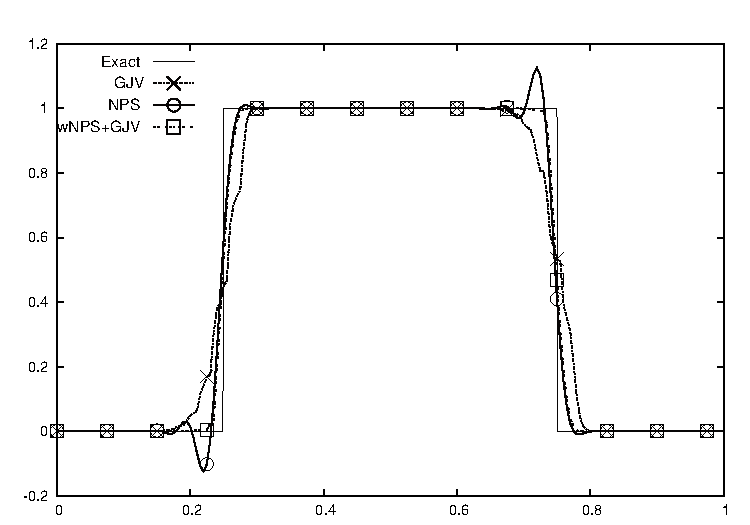
\includegraphics[width=9.65cm]{Figures/paper1/test20_p1_200.pdf}} %
\subfigure[Terracing effect.]{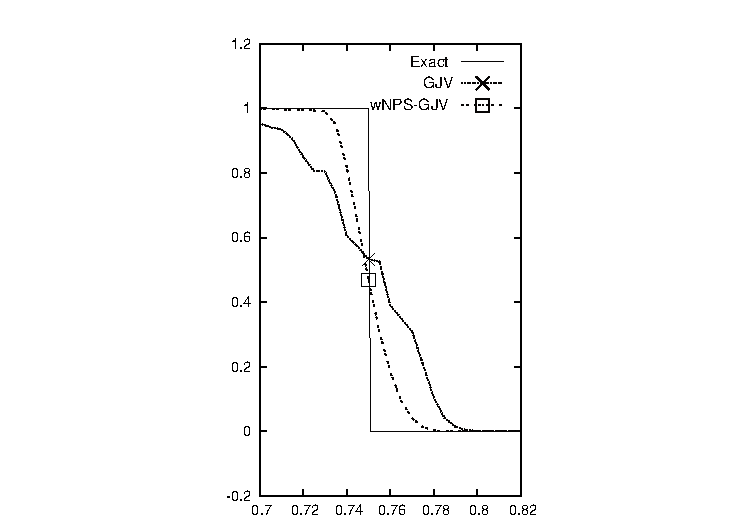
\includegraphics[clip=true, trim=3.8cm 0cm 3.1cm 0cm,width=4.35cm]{Figures/paper1/test20_p1_200_d2.pdf}} %
\caption{$1D$ pulse under transport equation. GJV ($c_{\rm gjv}=0.5$, $q=10$); $p=1$; $N=200$; Crank-Nicolson (CFL$=0.5$); no mass lumping.}\label{fig-pulse1}
\end{figure}

The same test can be used to check the dependence of the DMP property on the variable $c_{\rm gjv}$ in the transport problem.  For this test, we have used the explicit forward Euler method for the integration in time with mass lumping and a CFL of $0.01$ in such a way that the error of the integration in time can be neglected. \Fig{SZ_AD_2} shows the results obtained when solving problem \Eq{eqtr}-\Eq{trinc} with  wNPS-GJV in Algorithm \ref{alg-wNPS-GJV}. We notice that the larger the value of $q$ the sharper are the oscillations that appear for $c_{\rm gjv} < 0.5$, so we have used $q=100$ to show the results. It is clear that the threshold $c_{\rm gjv} = 0.5$ is sharp; overshoots and undershoots appear in the solution when $c_{\rm gjv}$ is slightly smaller than $0.5$, violating the TVD property.
\begin{figure}%
\centering
\subfigure[$c_{\rm gjv}  = 0.49,0.5,0.51$]{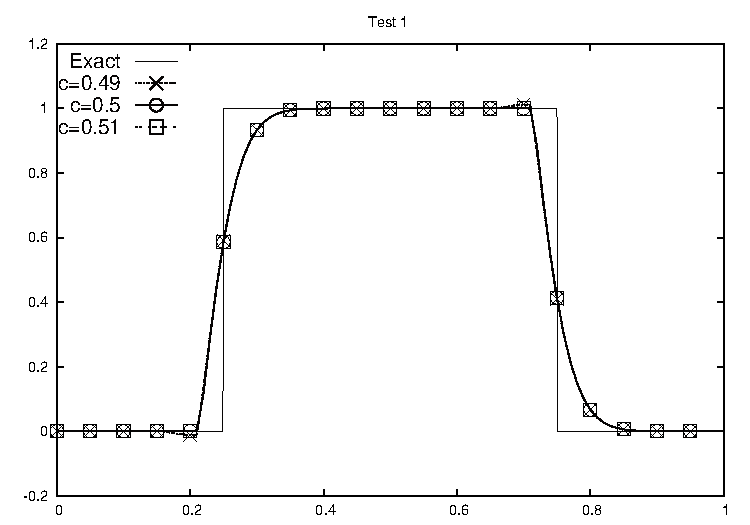
\includegraphics[width=7cm]{Figures/paper1/BurmanSZ.pdf} %
\label{fig-SZ_AD_2_s1} }%
\subfigure[Detail of \subref{fig-SZ_AD_2_s1}]{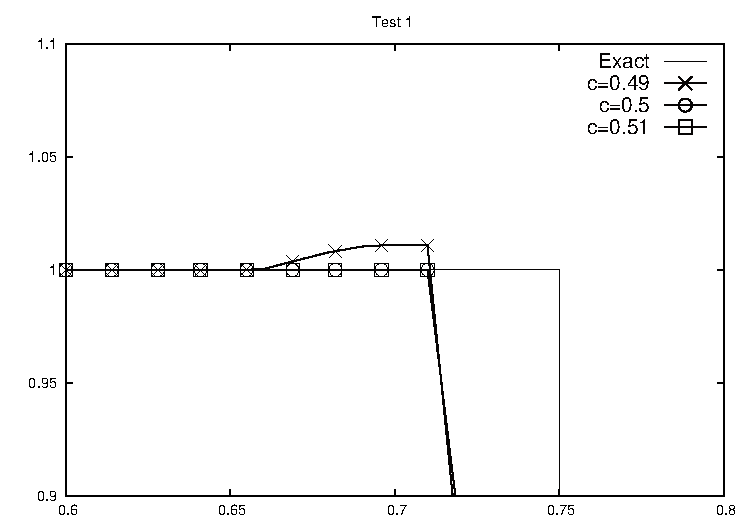
\includegraphics[width=7cm]{Figures/paper1/BurmanSZ1d.pdf}  }%
\caption{$1D$ pulse under transport equation. GJV ($c_{\rm gjv}=0.5$, $q=100$); $p=1$; $N=100$; forward Euler (CFL$=0.01$); mass lumping.}\label{fig-SZ_AD_2}%
\end{figure}


\subsection{Test 2: Convergence to a smooth solution}

In order to check that the order of convergence is not affected by the stabilization added, we will evaluate the error reduction for a sinusoidal when refining the mesh. The test consists in solving the 2$D$ transport equation \Eq{probcont} with $\beta = (1,0)$, $f=0$, initial solution $u_0(x,y) = \sin(2\pi x)$ in $\Omega=[0,1]\times[0,1]$ and periodic boundary conditions in the $x$ direction. The solution presents  maximum and minimum values along two lines ($x=\frac{1}{4}$ and $x=\frac{3}{4}$ respectively for $t=0$) that activate the shock-capturing. The desired behaviour is that this activation does not affect the convergence of the method. The meshes used for the test are regular triangular meshes of size $N_h\times N_h(\times 2)$. The $L^2(\Omega)$ errors are plotted in \Fig{smooth_sol}. The label $cG$ stands for the continuous Galerkin scheme without any stabilization and is the reference for the desired convergence one wants to attain when solving smooth solutions. It is clear that the convergence order is spoiled when using shock-capturing techniques without any linear stabilization, specially when using the bGJV method. On the other hand the convergence is maintained when both methods are combined with linear stabilization, either wNPS or SUPG. This test provides another motivation to combine linear and nonlinear stabilization, i.e., to have superior convergence in smooth regions.

\begin{figure}
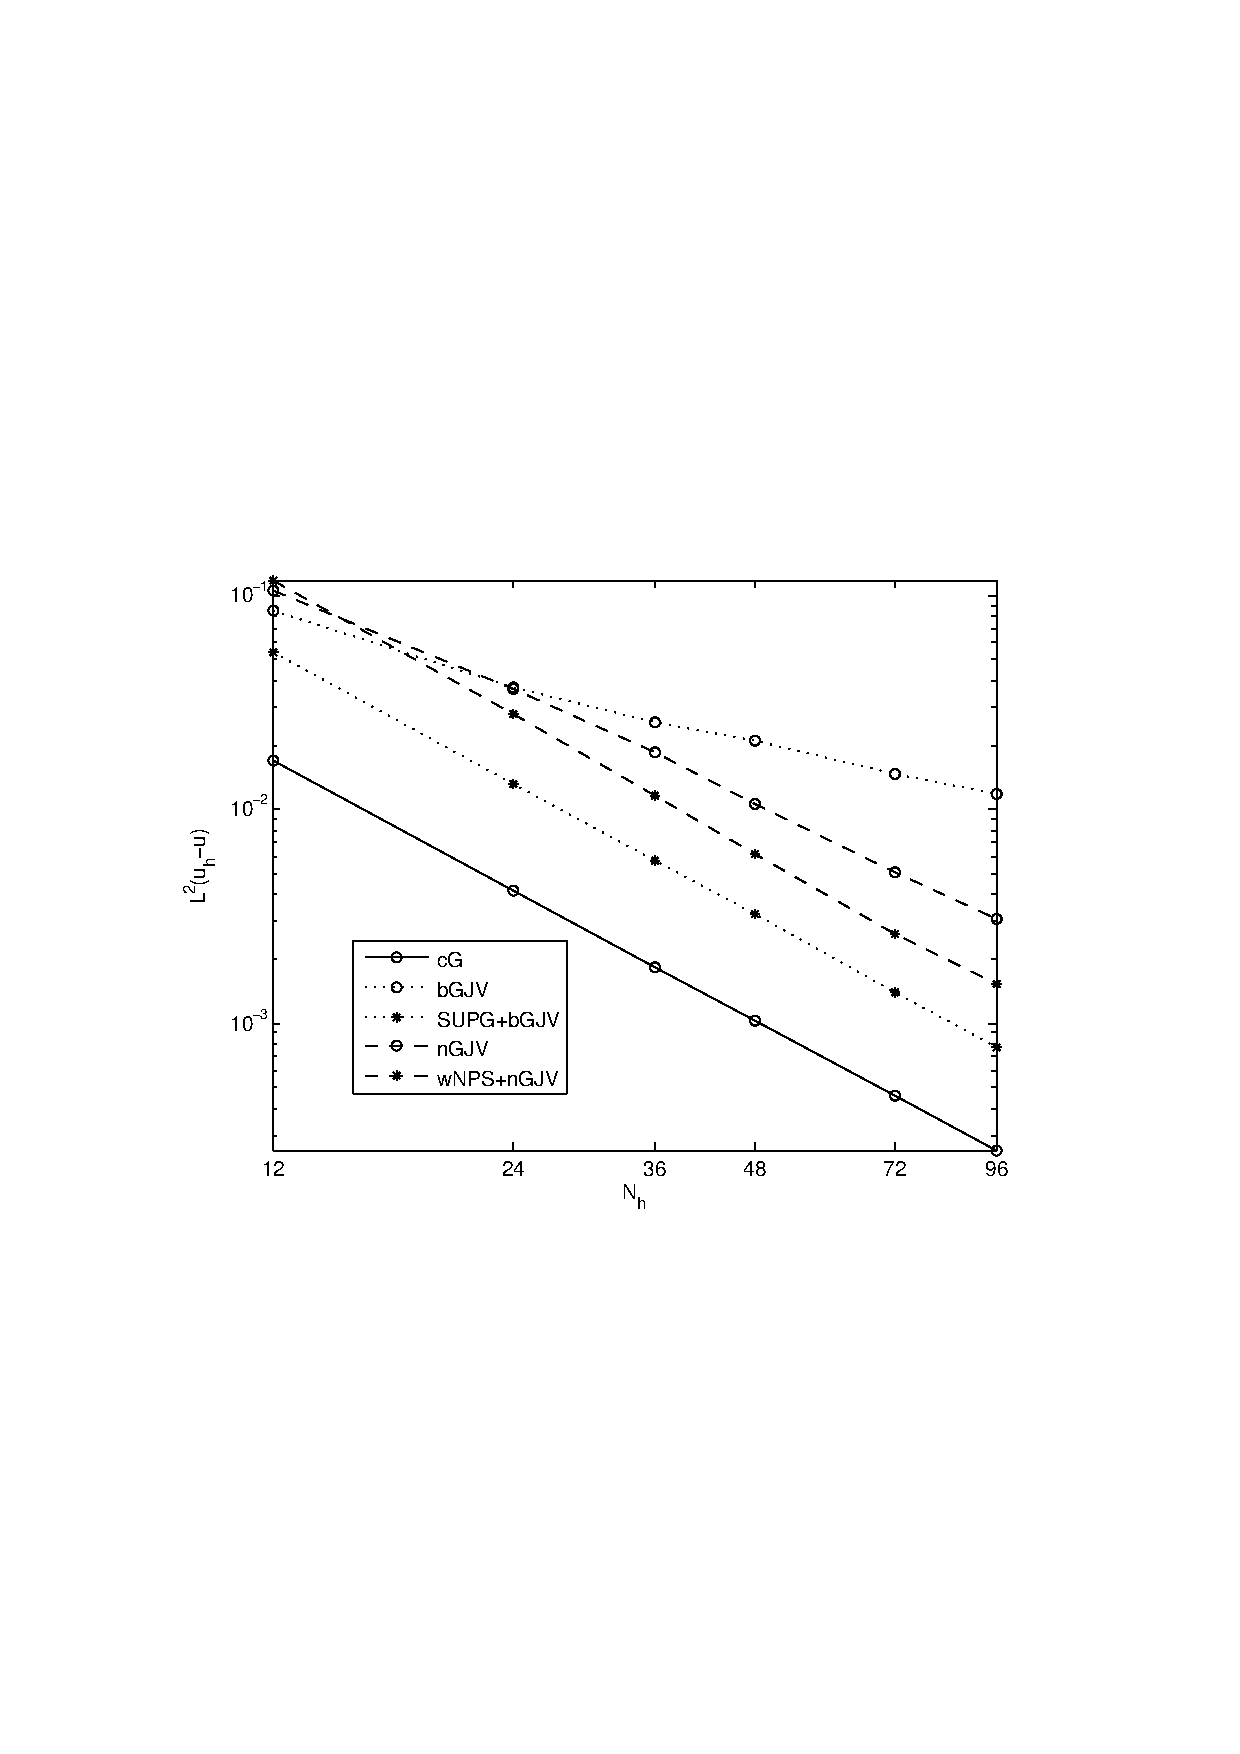
\includegraphics[clip=true, trim=0cm 9cm 0cm 9cm,width=14cm]{Figures/paper1/smooth_conv_test_2D.pdf}%
 \caption{Smooth solution. $L^2(\Omega)$ error vs size of the mesh. Crank-Nicolson; $t=1$; $\Delta t = 10^{-3}$; no mass lumping.}\label{fig-smooth_sol}
 \end{figure}

\subsection{Test 3: Multidimensional transport problem} 
Now, we want to show the performance of nGJV and bGJV nonlinear stabilization for multidimensional problems. We solve the $2D$ transport equation \Eq{eqtr} in $\Omega = [0,1]\times[0,1]$ with $\bb=(-2\pi (y-0.5), 2\pi (x-0.5))$. The initial solution is given in \cite{dmitri_kuzmin_guide_2010} and its interpolation in a mesh of $250\times250$ bilinear elements is displayed in \Fig{kuzmin0}. %We have extended the definition of the amount of artificial viscosity as it is shown in \Eq{gjvisc}. 
 

\begin{figure}%
\centering
\subfigure[Nodally exact initial solution]{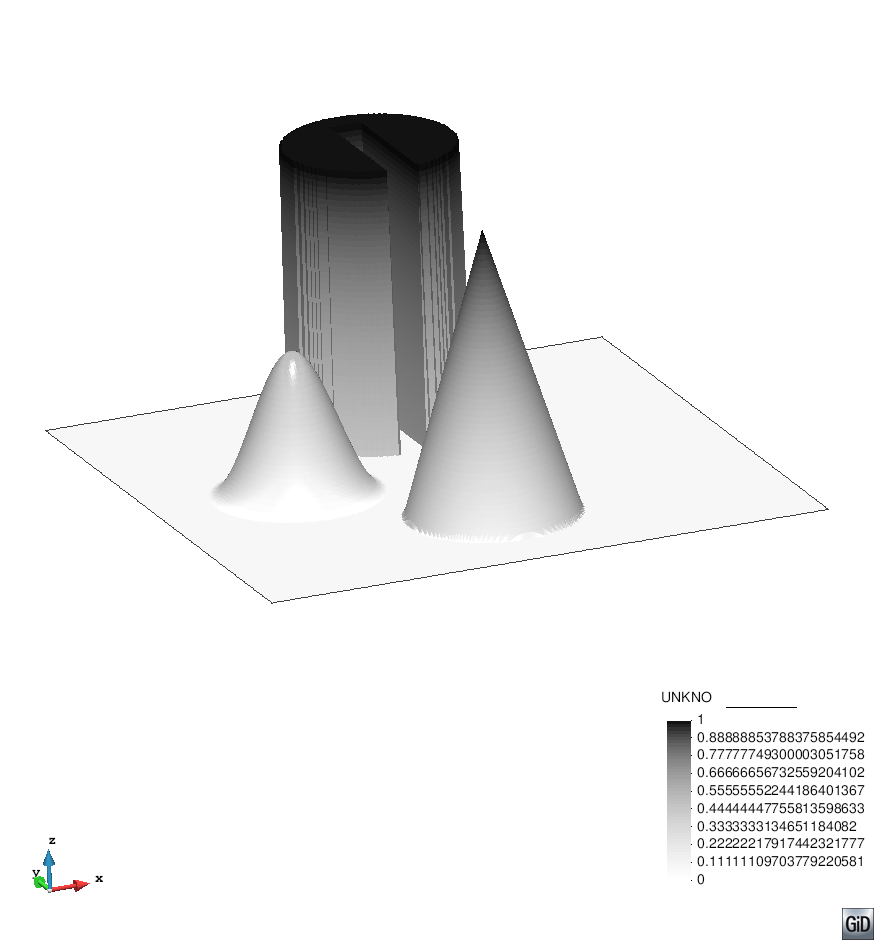
\includegraphics[clip=true, trim=1.6cm 11cm 1.6cm 3cm,width=7.0cm]{Figures/paper1/inisol.png}\label{fig-kuzmin0}}%
\subfigure[Error regions]{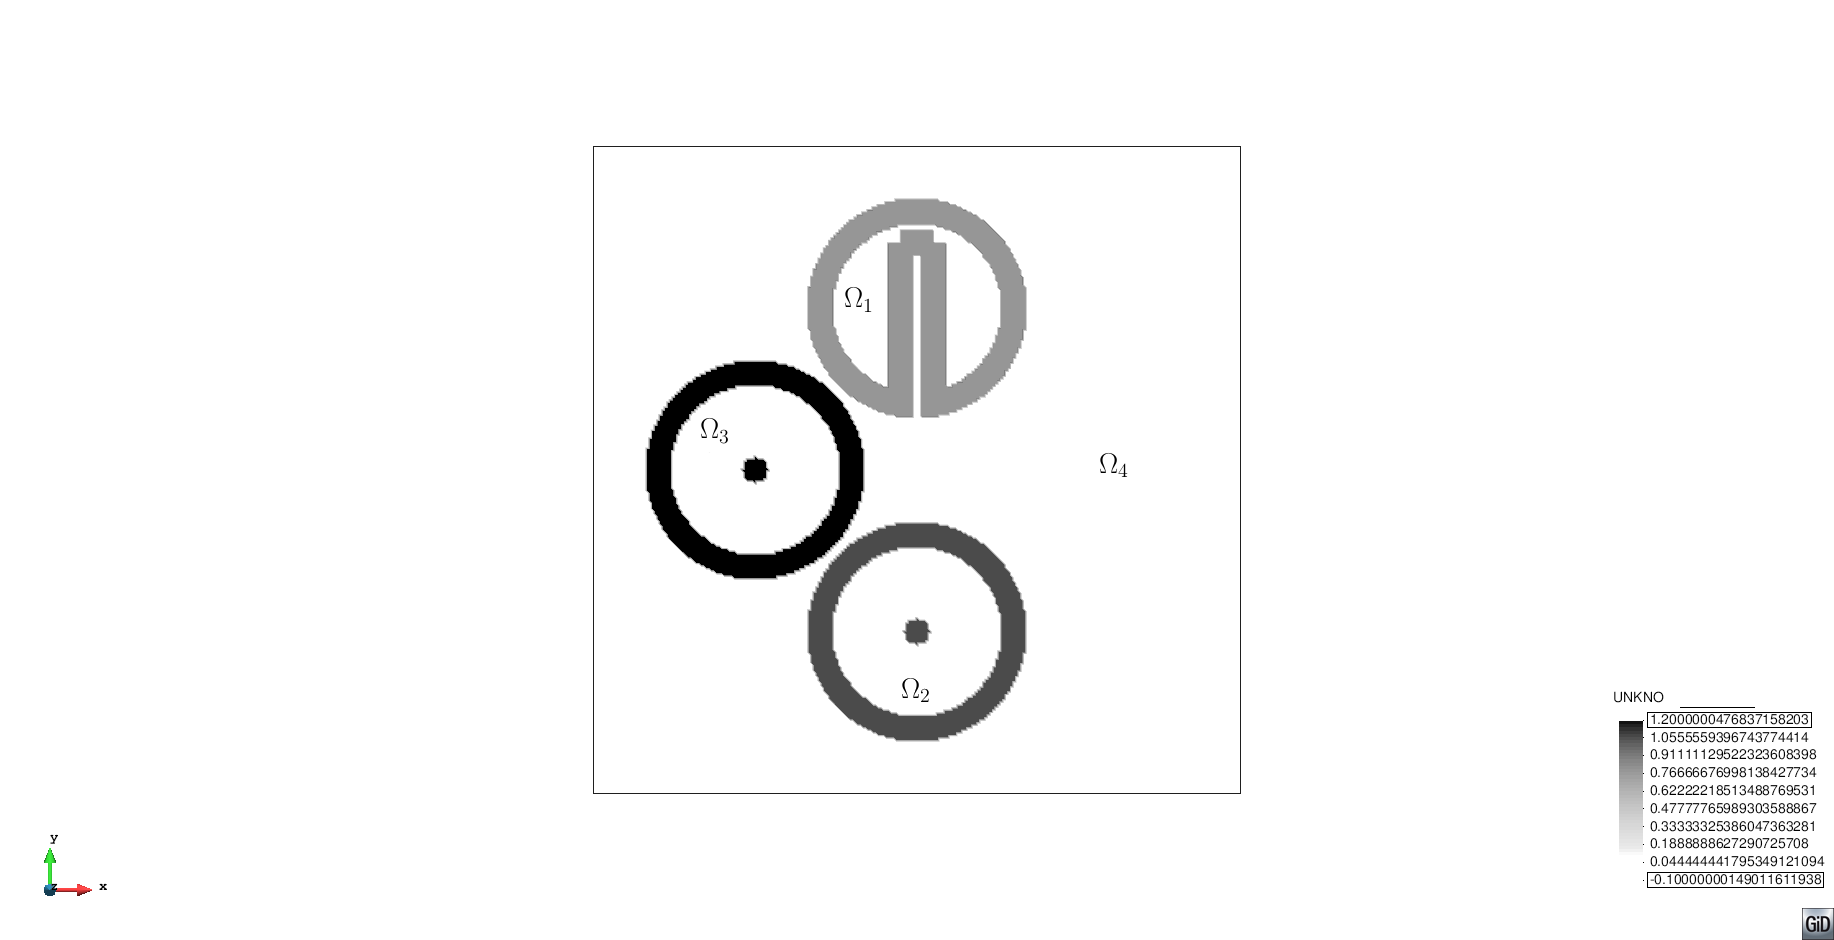
\includegraphics[clip=true, trim=15cm 4cm 15cm 4cm,width=7.0cm]{Figures/paper1/error_regions.png}\label{fig-err_reg}}
\caption{Three body rotation. Nodally exact initial solution and error regions.}\label{fig-algo}
\end{figure}


The solution is computed until $t=1$ with a $250 \times 250 (\times 2)$ triangular mesh. Crank-Nicolson with time step $\Delta t = 2\cdot 10^{-4}$ and without mass lumping is used for the integration in time.  We compare the performance of nGJV and bGJV (with and without linear stabilization), EV, and RV  methods. The value of the constant of each method is specified in Algorithm \ref{alg-wNPS-GJV} and all of them have been optimized to obtain the best results. With regard to the EV formulation, we have considered the value of the constants following \cite{guermond_entropy_2011}.\footnote{Let us note that the results for the EV method have been obtained with the entropy function $\eta = (u- 1/2)^2$. This choice is basic to reproduce these results, since the discontinuities under consideration have plateaus on $u = 0$ and 1, and the use of $\eta = u^2$ or $\eta = (u-1)^2$ leads to worse results.} 
An approximation of the $L^2$ error after one cycle has been computed in $4$ different regions $\Omega_1$, $\Omega_2$, $\Omega_3$, $\Omega_4$ that are plotted in \Fig{err_reg}. The first $3$ regions consist of a layer of width $2\cdot 10^{-2}$ around the regions where the function or its gradient change abruptly. The results are collected in Table \ref{tab-ex15_malla2D_new}. Most of the error is concentrated in $\Omega_1$, the layer around the cylinder. In general all the methods give a similar order of error in each region and there is no method that clearly outstands from the rest.
However, the numerical results obtained with the different methods are certainly different, as one can observe in the actual results plotted in \Fig{triangle1} at $t = 1$. The solutions obtained with nGJV are oscillation-free up to solver tolerance error. Even though the nGJV method without stabilization gives the smallest error in $\Omega_1$, the terracing effect can be appreciated around the cylinder. When wNPS stabilization is added, the solution is smoothed in the region. The strongest oscillations are observed in the SUPG-RV solution. The EV solution presents oscillations on the $u_h=0$ plateau around the shapes that cannot be clearly observed in the plot, and these oscillations become larger when the problem is solved with a quadrilateral mesh. 
\begin{table}
\centering
\begin{tabular}{lccccc}
\hline
Method &  $\Omega_1$ &  $\Omega_2$ &  $\Omega_3$ &  $\Omega_4$\\\hline
wNPS + bGJV  &  2.961e-01 & 1.338e-02
&  3.071e-03
&  1.033e-02\\

SUPG + bGJV  &
  2.698e-01    
  & 1.234e-02
  & 2.303e-03
  & 8.929e-03 \\
    None + EV  &
  2.854e-01     
&  9.123e-03
&  8.412e-04
&  1.287e-02\\

SUPG + RV  &
  2.634E-01     
&  7.551e-03
&  2.063e-03
&  6.933e-03 \\
nGJV  &
  2.318e-01     
&  1.015e-02
&  1.914e-03
&  6.957e-03\\

wNPS + nGJV  &
  2.848e-01     
&  1.119e-02
&  1.546e-03
&  7.834e-03\\
\hline
\end{tabular}
\caption{Three body rotation. $\|u-u_h\|_{\Omega_i}$}\label{tab-ex15_malla2D_new}
\end{table}
\begin{figure}%
\centering
\subfigure[{ wNPS-bGJV}]{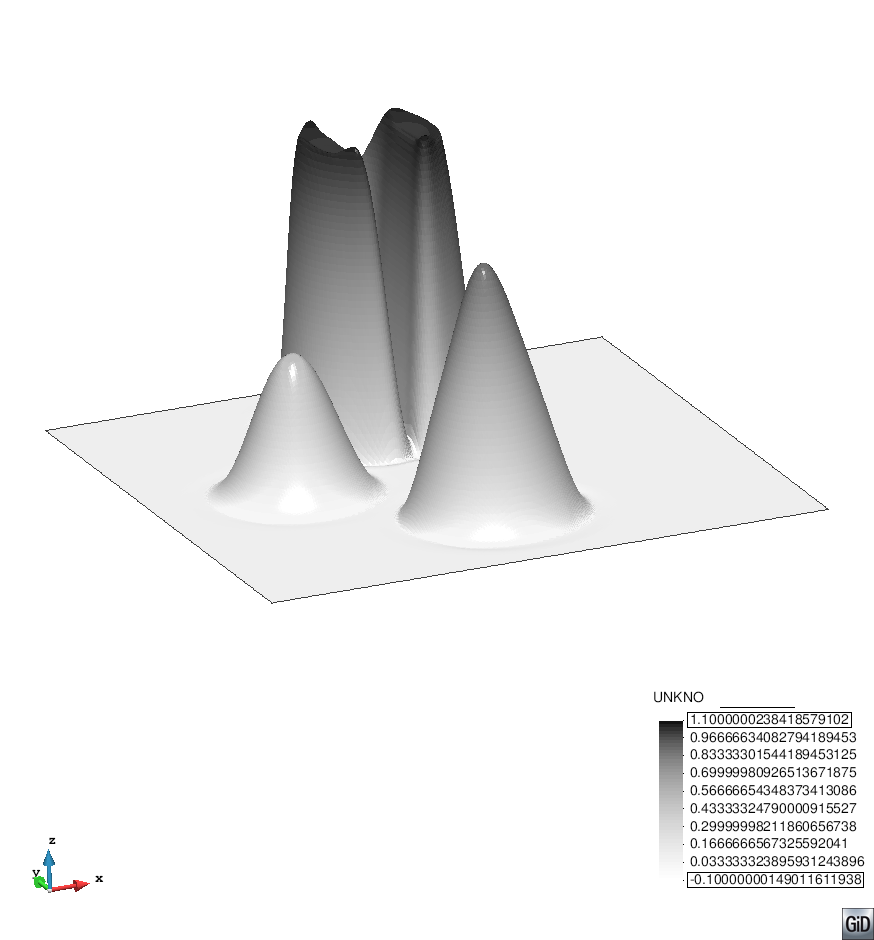
\includegraphics[clip=true, trim=1.6cm 11cm 1.6cm 3cm,width=0.5\textwidth]{Figures/paper1/15_SZ_GJV_T.png}}%
\subfigure[{SUPG-bGJV}]{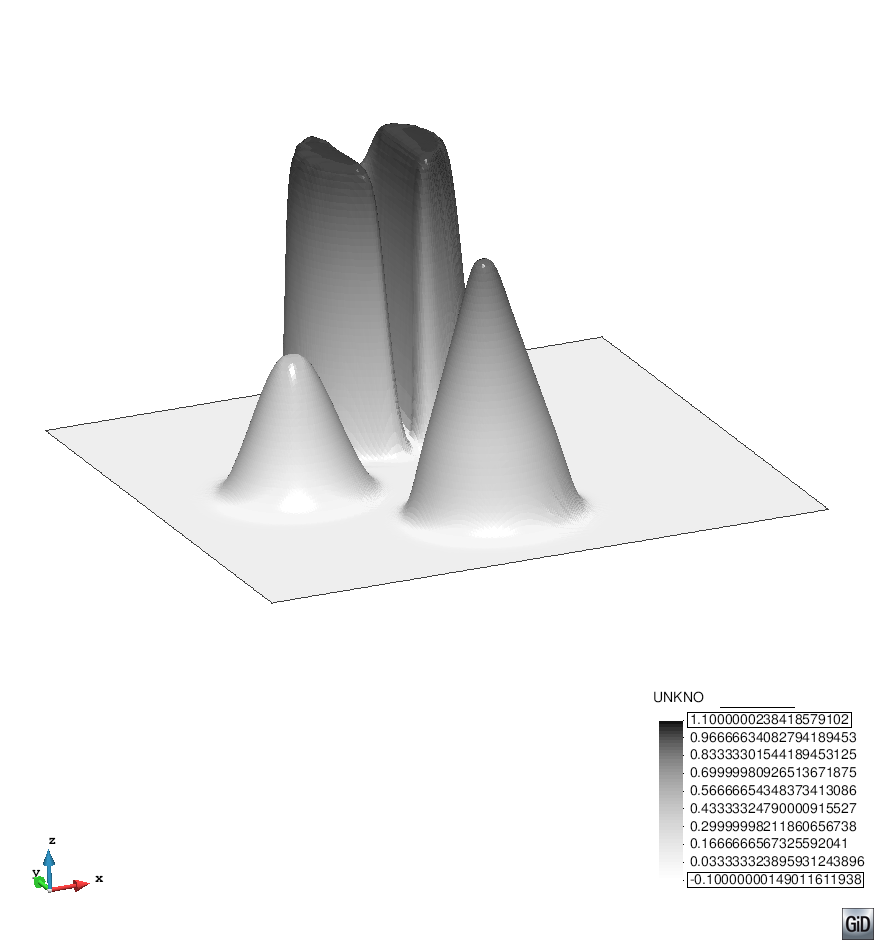
\includegraphics[clip=true, trim=1.6cm 11cm 1.6cm 3cm,width=7.0cm]{Figures/paper1/15_SUPG_GJV_T.png}\label{fig-sq1-supgbgjv}}\\
\subfigure[{EV}]{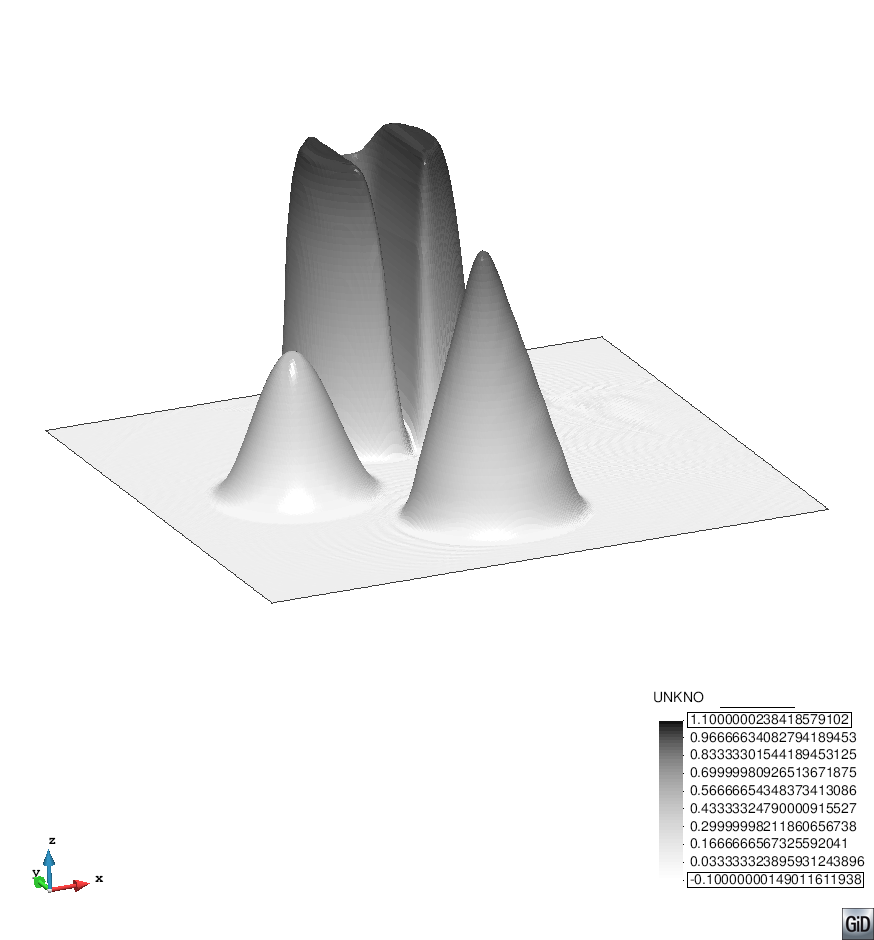
\includegraphics[clip=true, trim=1.6cm 11cm 1.6cm 3cm,width=7.0cm]{Figures/paper1/15_None_EV_T.png}}%
\subfigure[{SUPG-RV}]{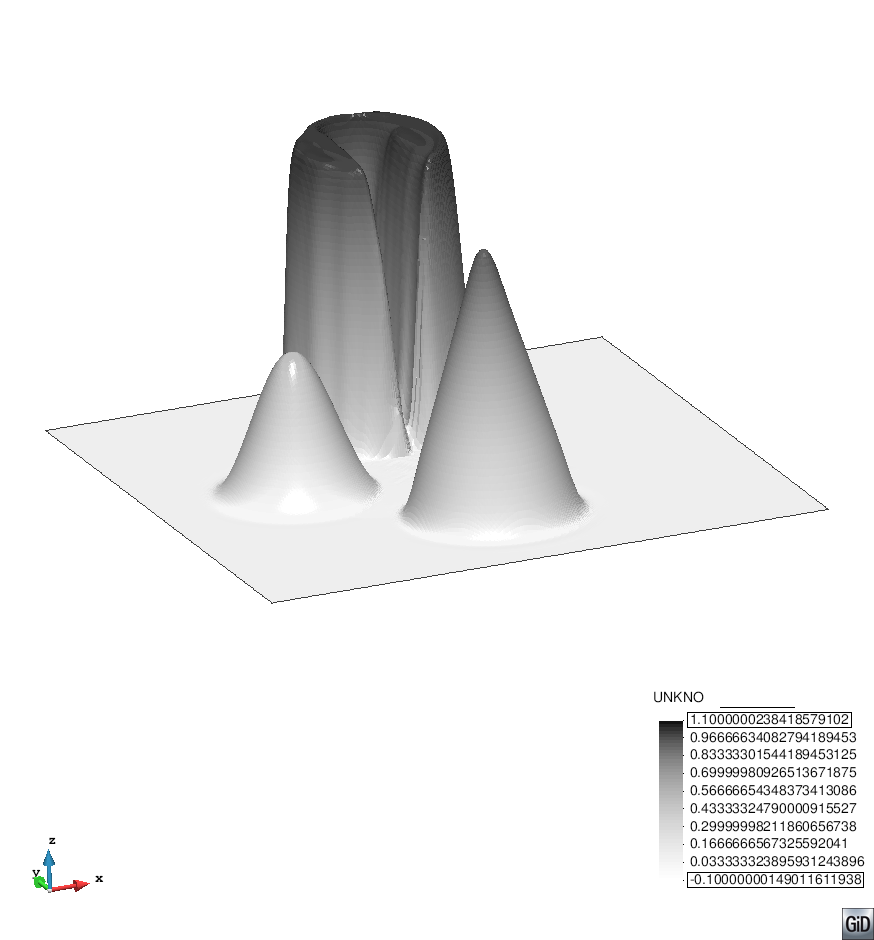
\includegraphics[clip=true, trim=1.6cm 11cm 1.6cm 3cm,width=7.0cm]{Figures/paper1/15_SUPG_RV_T.png}}\\
\subfigure[{nGJV}]{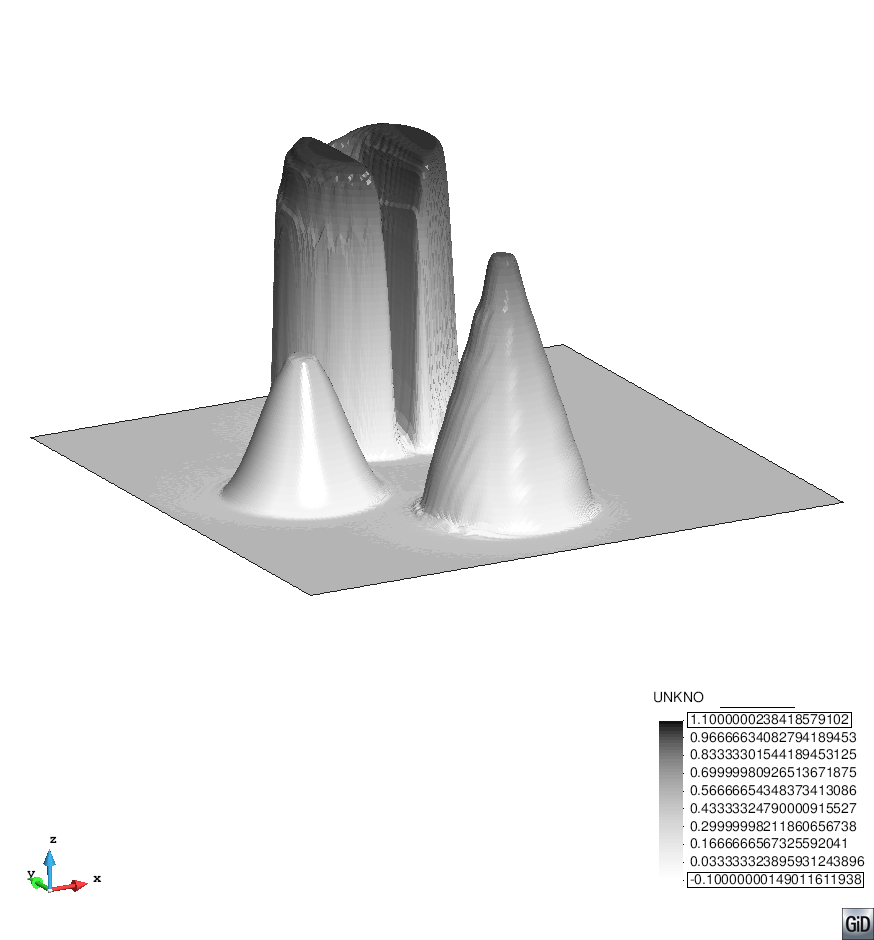
\includegraphics[clip=true, trim=1.6cm 11cm 1.6cm 3cm,width=7.0cm]{Figures/paper1/15_None_PGJV_T.png}}%
\subfigure[{ wNPS-nGJV}]{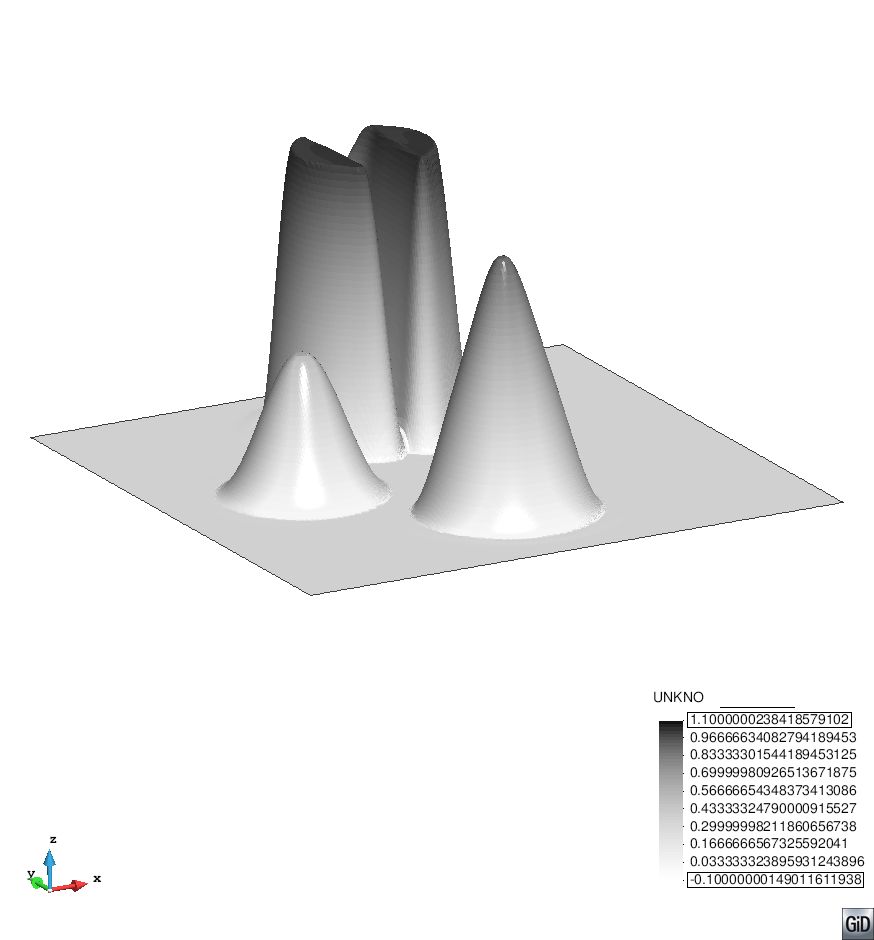
\includegraphics[clip=true, trim=1.6cm 11cm 1.6cm 3cm,width=7.0cm]{Figures/paper1/15_SZ_PGJV_T.png}}
\caption{ Three body rotation. Results for different methods. $p=1$; $250\times 250 (\times 2)$ triangular mesh; Crank-Nicolson; $t=1$; $\Delta t = 2 \cdot 10^{-4}$; no mass lumping.}\label{fig-triangle1}
\end{figure}

The results reported in \Fig{triangle1} are at the final stage of the computation, i.e., $t=1$, and the oscillations have already been smoothed out. In order to better evaluate how the different methods succeed eliminating oscillations, we introduce the oscillation function
\begin{align*}
&{\rm osc}(t) = \max_{(x,y)\in \Omega} \left\{0 , u_h(x,y,t) - 1 , -u_h(x,y,t) \right\}.
\end{align*}
We compute the mean value of the parameter ${\rm osc(t)}$ in bunches of $50$ time steps and the time evolution of this quantity for the different methods is plotted in \Fig{osc}. It can be appreciated that the method with the smallest overshoots and undershoots is nGJV without any linear stabilization; when the wNPS is added, the order of the oscillations is still very low. We remark that the DMP is not exactly attained for the nGJV method since we are considering non-acute meshes, no mass lumping, and inexact time integration. bGJV shows smaller oscillations when combined with SUPG stabilization than with the wNPS; it is noticeable the good behavior of bGJV with SUPG compared to the traditional RV-SUPG approach. Focusing on the first time steps, where the stronger oscillations occur, RV and bGJV present strong violations of the DMP (either wiht SUPG and with wNPS linear stabilization). These oscillations remain for SUPG-RV and wNPS-bGJV methods during the whole computation. This oscillatory behaviour is clearly observed  in \Fig{osrv}, where we plot the solutions obtained  at time $t=0.01$. 

\begin{figure}%
\centering
\subfigure[${\rm osc(t)}$ in time]{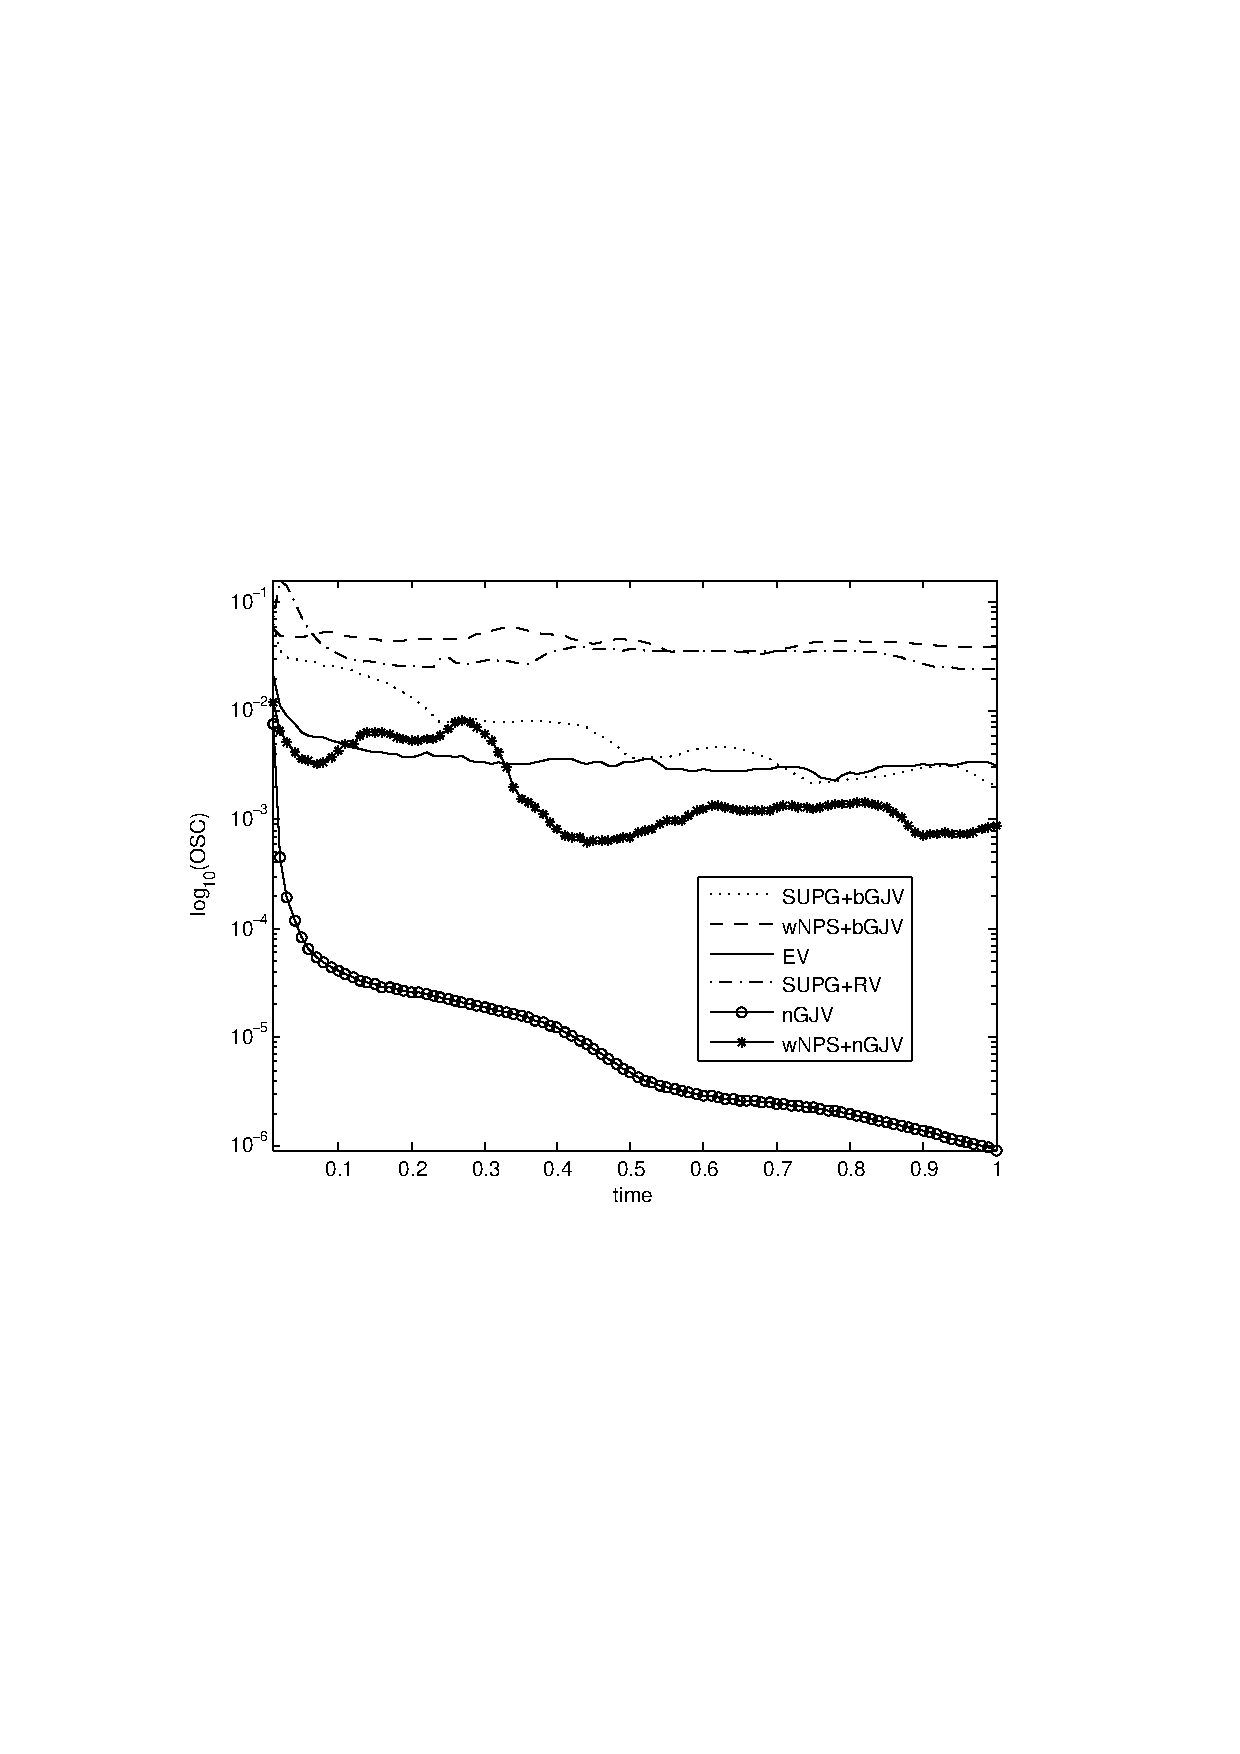
\includegraphics[clip=true,  trim=3cm 9cm 4cm 9cm,width=0.5\textwidth]{Figures/paper1/osc_time_tr.pdf}\label{fig-osc}}%
\subfigure[{SUPG-RV, $t = 0.01 $}]{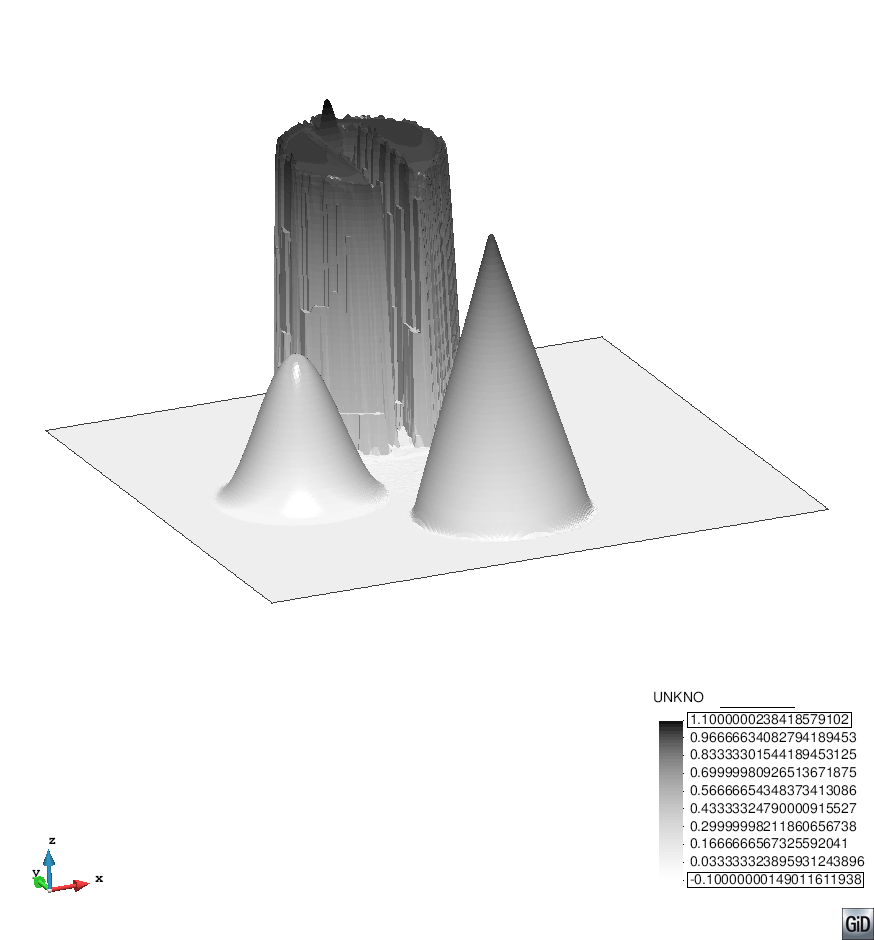
\includegraphics[clip=true, trim=1.6cm 11cm 1.6cm 3cm,width=0.5\textwidth]{Figures/paper1/15_SUPG_RV_T_001.png}\label{fig-osrv}}\\%
\caption{Three body rotation. Evolution of the oscillations in time. $p=1$; $250\times 250 (\times 2)$ triangular mesh; Crank-Nicolson; $t=1$; $\Delta t = 2 \cdot 10^{-4}$; no mass lumping.}\label{fig-osctime}
\end{figure}

Even when the analysis performed in this work has been done on simplicial meshes, the methods have been tested in quadrilateral meshes also. All the methods provide similar results in both kind of meshes with the notable exception of the bGJV method that, when combined with SUPG stabilization, leads to a very accurate approximation of the solution. The result is plotted in \Fig{gjvquad}. It is remarkable how the solution keeps the shape of the cylinder and the plateu $u_h=1$. We want to stress that a naive extension of the $1D$ method in \cite{burman_nonlinear_2007}, i.e., the artificial diffusion in \Eq{gjvisc} without the correction term $\frac{\int_e |\nabla u_h \cdot n|{\rm d} \sigma}{\int_e |\nabla u_h| {\rm d} \sigma}$, is extremely over-diffusive. The results after one cycle are displayed in \Fig{notuning}. We can observe the dramatic improvement obtained with the correction factor by comparing both plots.

\begin{figure}%
\centering
\subfigure[{SUPG-bGJV}]{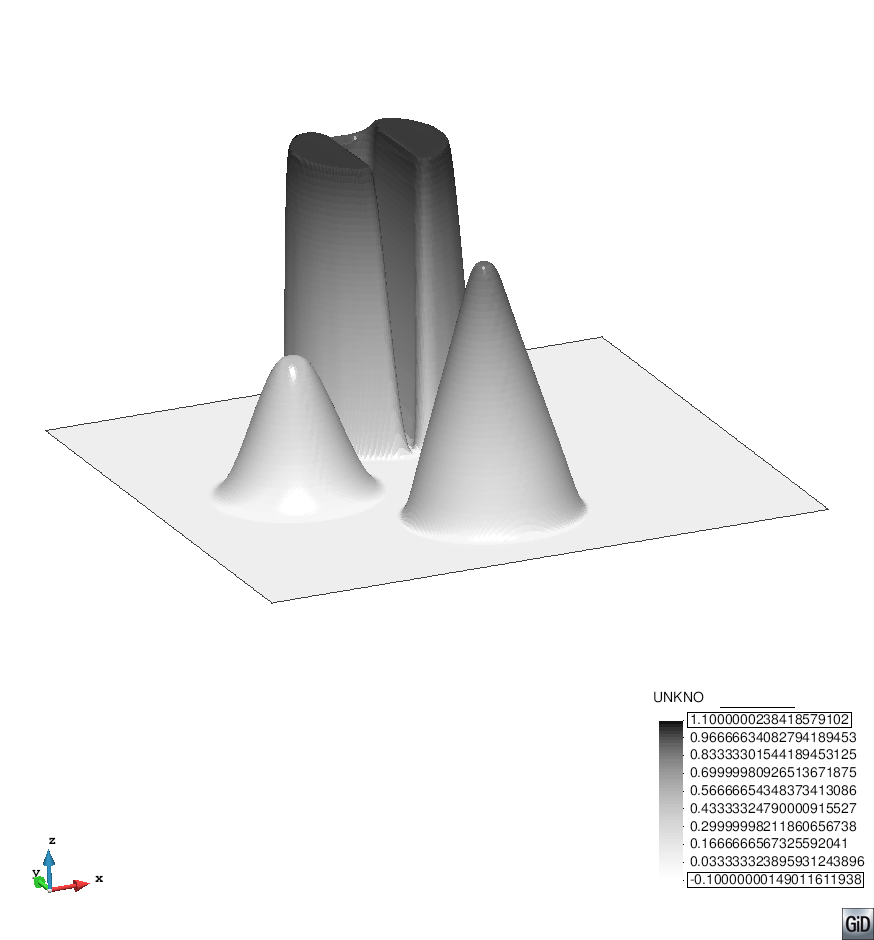
\includegraphics[clip=true, trim=1.6cm 11cm 1.6cm 3cm,width=0.5\textwidth]{Figures/paper1/15_SUPG_GJV_Q.png}\label{fig-gjvquad}}%
\subfigure[{SUPG-bGJV without correction}]{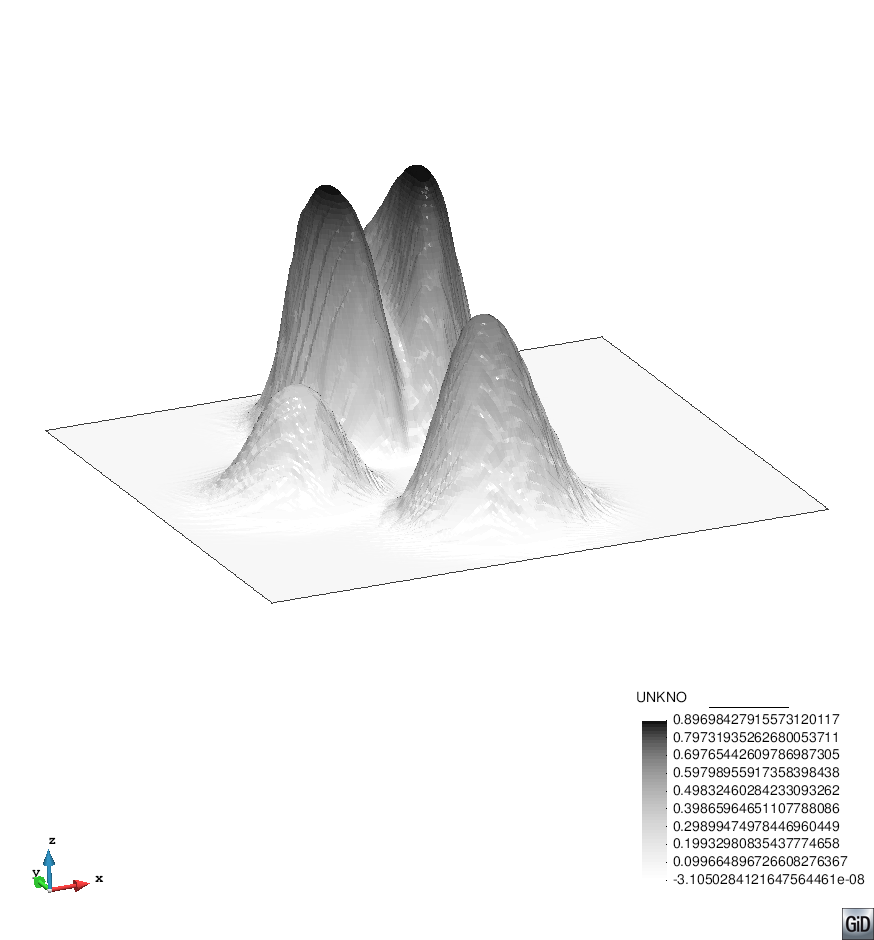
\includegraphics[clip=true, trim=1.6cm 11cm 1.6cm 3cm,width=0.5\textwidth]{Figures/paper1/15_SUPG_GJV_NOtunning.png}\label{fig-notuning}}
\caption{Three body rotation. The effect of the correction term. $p=1$; $250\times 250 (\times 2)$ triangular mesh; Crank-Nicolson; $t=1$; $\Delta t = 2 \cdot 10^{-4}$; no mass lumping.}\label{fig-square1}
\end{figure}

\section{Conclusions}\label{s-concl}
In this chapter we introduce the linear stabilization technique for continuous FE
discretizations of time-dependent transport problems which belongs to the family of local 
projection stabilization techniques. In particular, we consider a Scott-Zhang-type projector which is 
well-defined for $L^1(\Omega)$ functions, extending the ideas in \cite{badia_stabilized_2012} to convection stabilization. 
Stability and numerical analyses for the linear transport problem are carried out. 

Further, we design a weighting of the aforementioned linear stabilization such that, 
when combined with a FE discretization with a DMP (usually
attained via a shock-capturing technique), it does not spoil the monotonicity properties. 
It is attained by switching off the linear stabilization around shocks.

Next, we have proposed different nonlinear stabilization (shock-capturing) schemes based on 
artificial viscosity, in order to reduce or even eliminate local oscillations around shocks/discontinuities. 
In particular, we have used a definition of the artificial viscosity based on boundary gradient jumps (bGJV),
following the original work of Burman in \cite{burman_nonlinear_2007}, and another one based on
nodal jumps (nGJV). For the nodal method, we have proved a salient strong DMP property for multidimensional 
time-dependent transport problems.

Finally, a complete set of numerical experiments is included. On one hand, we check experimentally
the theoretical monotonicity properties of the weighting formulations and the nonlinear stabilization. Next, gradient-jump shock-capturing methods (with different linear stabilizations) are compared against residual-based and entropy-based formulations, in order to show its performance. The results obtained with the nGJV scheme are remarkably good, with oscillation-free solutions in different tests.
